\documentclass[twocolumn, a4paper]{article}
\usepackage[top=1cm, bottom=1.2cm, left=1.5cm, right=1.5cm]{geometry}
\usepackage{graphicx}
\usepackage{multirow}
\usepackage{float}
\usepackage{amsmath}

% \setlength\intextsep{0pt}
% \setlength{\columnsep}{0.6cm}

\begin{document}
\title{
	   \LARGE\textbf{Third Assignment ORC\\DQN Network}
	   \vspace{1cm}
	  }
\author{
		\textbf{Bertelli Davide} \\
		mat. 223718 \\
		davide.bertelli-1@studenti.unitn.it
		\and
		\textbf{Hueller Jhonny} \\
		mat. 221254\\
		jhonny.hueller@studenti.unitn.it
	   }
\date{}
\maketitle

\section{Abstract}
The third assignment revolved around the task to implement a deep Q-Learning
algorithm able to proficiently tackle the task to balance a pendulum.
This work focuses on the adaptation of the work in \cite{Mnih} to a simpler
environment, along with many suggestion from [IMPLEMENTING Q-NETWORK] for
implementing the details.
The resulting deep neural network is able to accurately estimate the Q-function
of the pendulum, and along with a greedy policy it produces episodes with
low cost, managing to balance the pendulum starting from any state.

\section{Introduction}
The pendulum is simulated having a continuous state space, which represents
the position and velocity of its joint variables, and a discrete control
space, which represents the joint torques requested by the controller.
Given this circumstances it is not possible to execute traditional Q-learning
and produce the Q-table necessary for estimating the Q-function, being the table
incompatible with continuous state spaces.
This is one of the reasons it might be preferable, if not required, to use
V/Q-function approximation techniques.
As instructed by [CITATION 2], In this work the Q-function has been approximated
using a deep neural network, which forced to implement several new components
into the training in order to ensure a good convergence.

\section{Components of Deep Q-Network}
The deep Q-learning algorithms introduces 3 majaor components: a deep neural network used to approximate the Q function, the use of mini-batches and experience replay in order to aid the proper execution of stochastic gradient descent, and the use of old network parameters in order to estimate the Q target for the loss function[INSERT CITATION 2].
Another important component, one which is not exclusive to deep Q-network, is the policy used for learning the Q-function.

\section{Network}
The network in use is composed of several fully connected layers which receive
as input the state of the pendulum, as mentioned before the position in
radiants and the angular velocity of each joint.
The last output layer produces the predicted Q value for each possible control
of the joints in the specific state.
Specifically the network is composed of: input layer, 4 dense hidden layers
having respectively 16, 32, 64 and 64 activation cells, and the output layer
having dimension equal to the number of discrete controls.
The number of controls is \(|U|=resolution^{\#joints}\), which
means that as \(resolution=15\) and \(\#joints=2\), \(|U|=15^{2}=225\) .
[REDO IMAGE]
In Figure \ref{fig:Network} is shown a graphical representation of the network
in use.

\label{fig:Network}
\begin{figure}
	\centering
	\includegraphics[width=8.5cm]{"../Figures/Network_schema"}
	\caption{Network architecture in case of $n\_joints$ composing the pendulum
			 and a control discretization over 11 steps.}
\end{figure}

\section{Loss, Experience Replay, Policy}
The traning loss uses the common least squares method between the target \(Q^{-}\) values, produced using the current cost and the discounted minimum estimated cost of the next state using old network parameters, and the current \(Q\) value, produced by the up-to-date network parameters: \(L(Q^{-},Q)=\sum_{i}(c_{i}+\gamma\min_{u'}Q^{-}(x_{i+1},u')-Q(x_{i},u_{i}))^{2}\).
The necessary data for the loss function, like state and control, are obtained using experience replay.
Experience replay is a technique used in order to remove the correlation between sequences of data.
Being \((x_{i}, u_{i}, c_{i}, x_{i+1})\) respectively the state, control, cost, and next state of the system at time \(i\), the experience replay buffer is composed of the list of transitions \({t_{i}=(x_{i}, u_{i}, c_{i}, x_{i+1}) \forall i\in [n, n+s)}\) the system produced during training and from which we randomly sample a mini-batch to be used for stochastic gradiant descent.
As the experience replay buffer has a limited size \(s\leq maximum\:size\) old transitions are progressively removed as new transitions are added when the size limit is reached.


\section{System setup}
The system provided as solution is composed by several objects:
\begin{itemize}
	\item \textbf{Buffer}: It is the object responsible to store the examples
		used by the actor network to train. Only the most recent examples are
		retained over the training to avoid that the actor network will learn
		a too old configuration of the system.
	\item \textbf{Policy}: It is the object responsible to chose the best
		control with which to feed the robot and allowing the movement among
		states.
	\item \textbf{Actor Network}: It is the network which has to be trained
		ov the environment and which output represents the Q Value obtained
		through the experience replay and exploration tasks.
	\item \textbf{Critique Network}: It is the target network which knows the
		environment and which is used to judge how well the actor network
		behaves. Its weights are fixed and it is not subjected to training. 
\end{itemize}
\subsection{Actor Network training}
The training of the network is carried on using the Mean Squared Error of the
Q Values provided by the network as the loss function which has to be
minimized and employing Adam as the optimizer.
To run the training the user is required to provide two mandatory values: the
number of episodes and the length of the episodes. These two parameters define,
respectively, the number of the random starting positions from which the 
robot will start the training and the length of the search executed for each
episode.
At each episode, and for all the length of the episodes, the buffer is randomly
sampled obtaining batches of tuples containing states, controls, next states
and costs. Then the provided batch is feeded to the Q network working as actor
and its output is feeded to the policy which will return the optimal control
for the next state, relying its judgment only on the Q Values provided, or it 
will try to explore the environment selecting a random control depending
by the probability set.
Once the policy had given its output the new control is applied to the robot
and the next state and cost are retrieved from the environment.
Having those informations, the states and controls, the next states and Q
Values, the actor network is feeded using the states and controls providing in
output its Q values. At this point the Q Values of the batch and those of the
actor network are used to compute the MSE representing our loss, lastly a
gradient update is performed.
Every 15 episodes the best network is saved by checking the average cost
among them.

\section{Actor Network testing}
The testing of the actor network was carried out first, varying the starting
position of the robot randomly and secondly making it start from the lowest
position to ensure the goodness of the results.
For each configuration three episodes were run and the sum of costs gathered
during their total length is used as the evaluation measure.
The testing phase works by gathering the robot state, querying the policy
for the next action, apply it and take the cost from the environment for all
the length of the episode.

\section{Experiments}
% 1 joint, 2 joints, N-joints
% Training time
% Changing resolution of the controls
The system has been tested over different configurations of the robot,
specifically with 1, 2 and more joints, different control resolution and
different number and length of episodes.
The evaluation metrics used are the loss of the training, the training time
and the total cost in the testing phase.

\section{Results}
\subsection{1 joint}
Following are shown the results in case the robot has 1 joint.

\label{fig:TrainLoss1}
\begin{figure}[H]
	\centering
	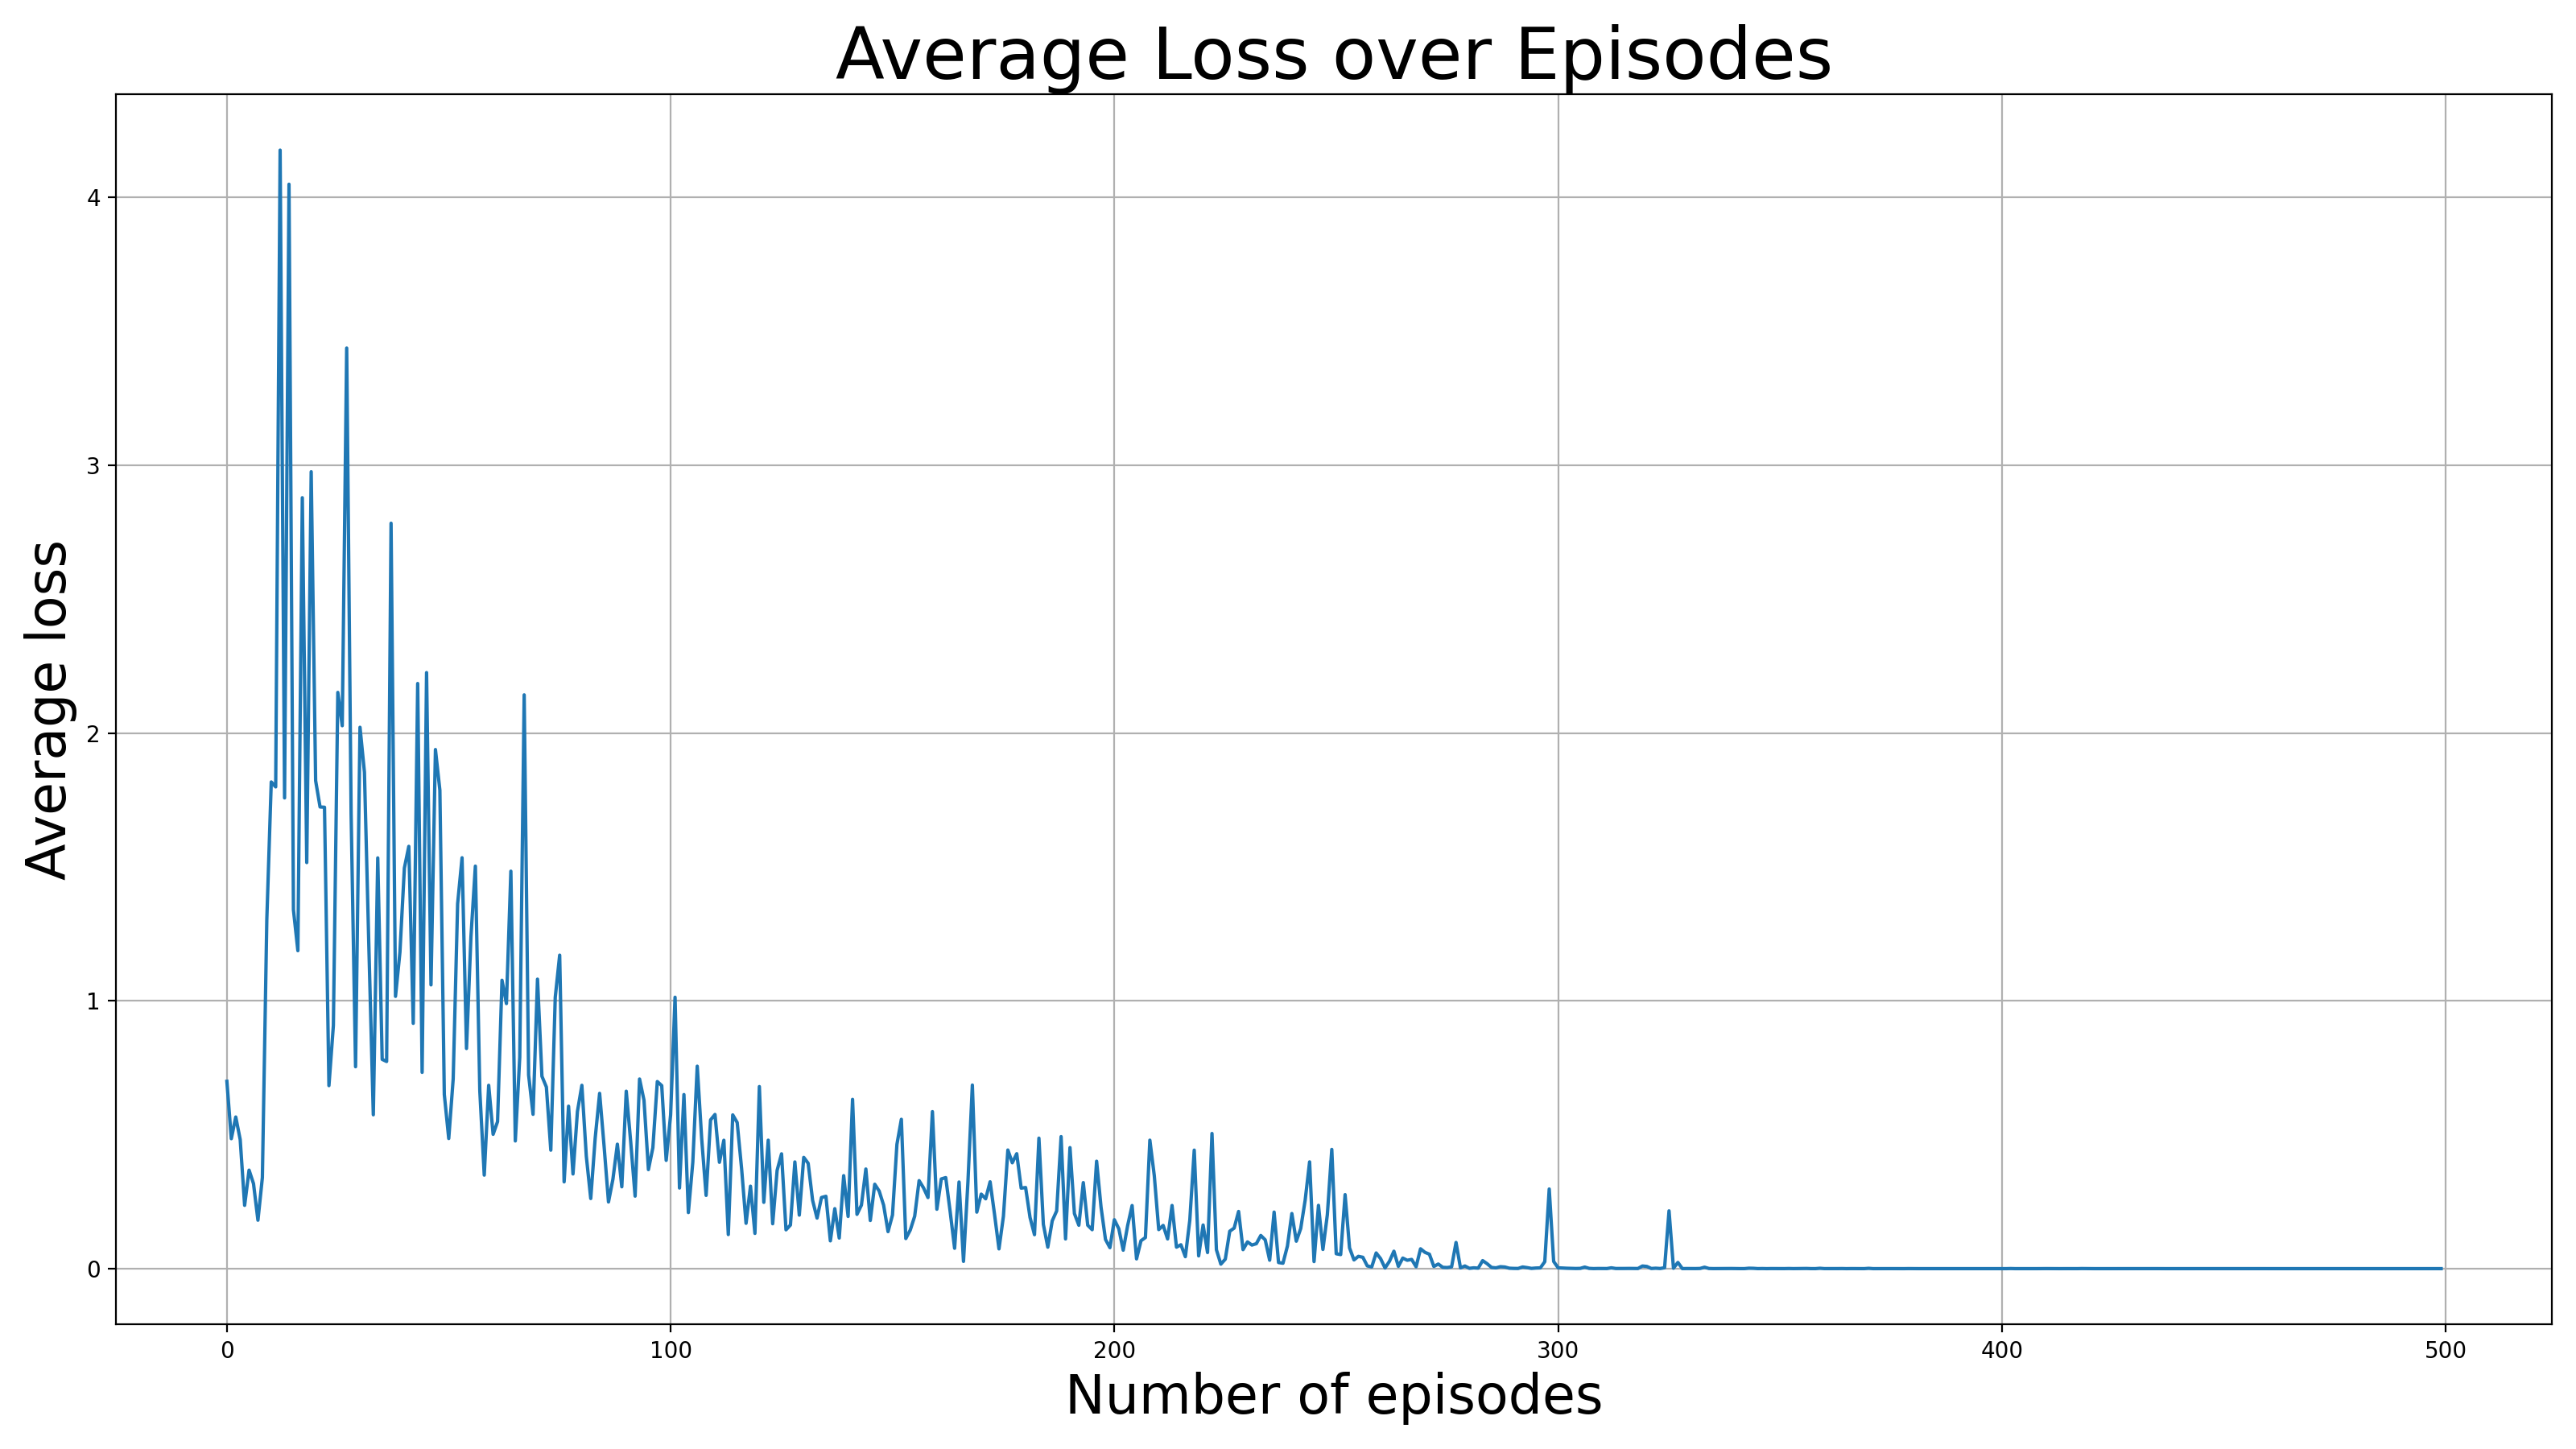
\includegraphics[width=8.5cm]{"../Figures/average_loss_over_epiodes_1J_500E_256EL.png"}
	\caption{Training loss having 1 joint.}
\end{figure}
\vspace{-1cm}
\label{fig:TrainTime1}
\begin{figure}[H]
	\centering
	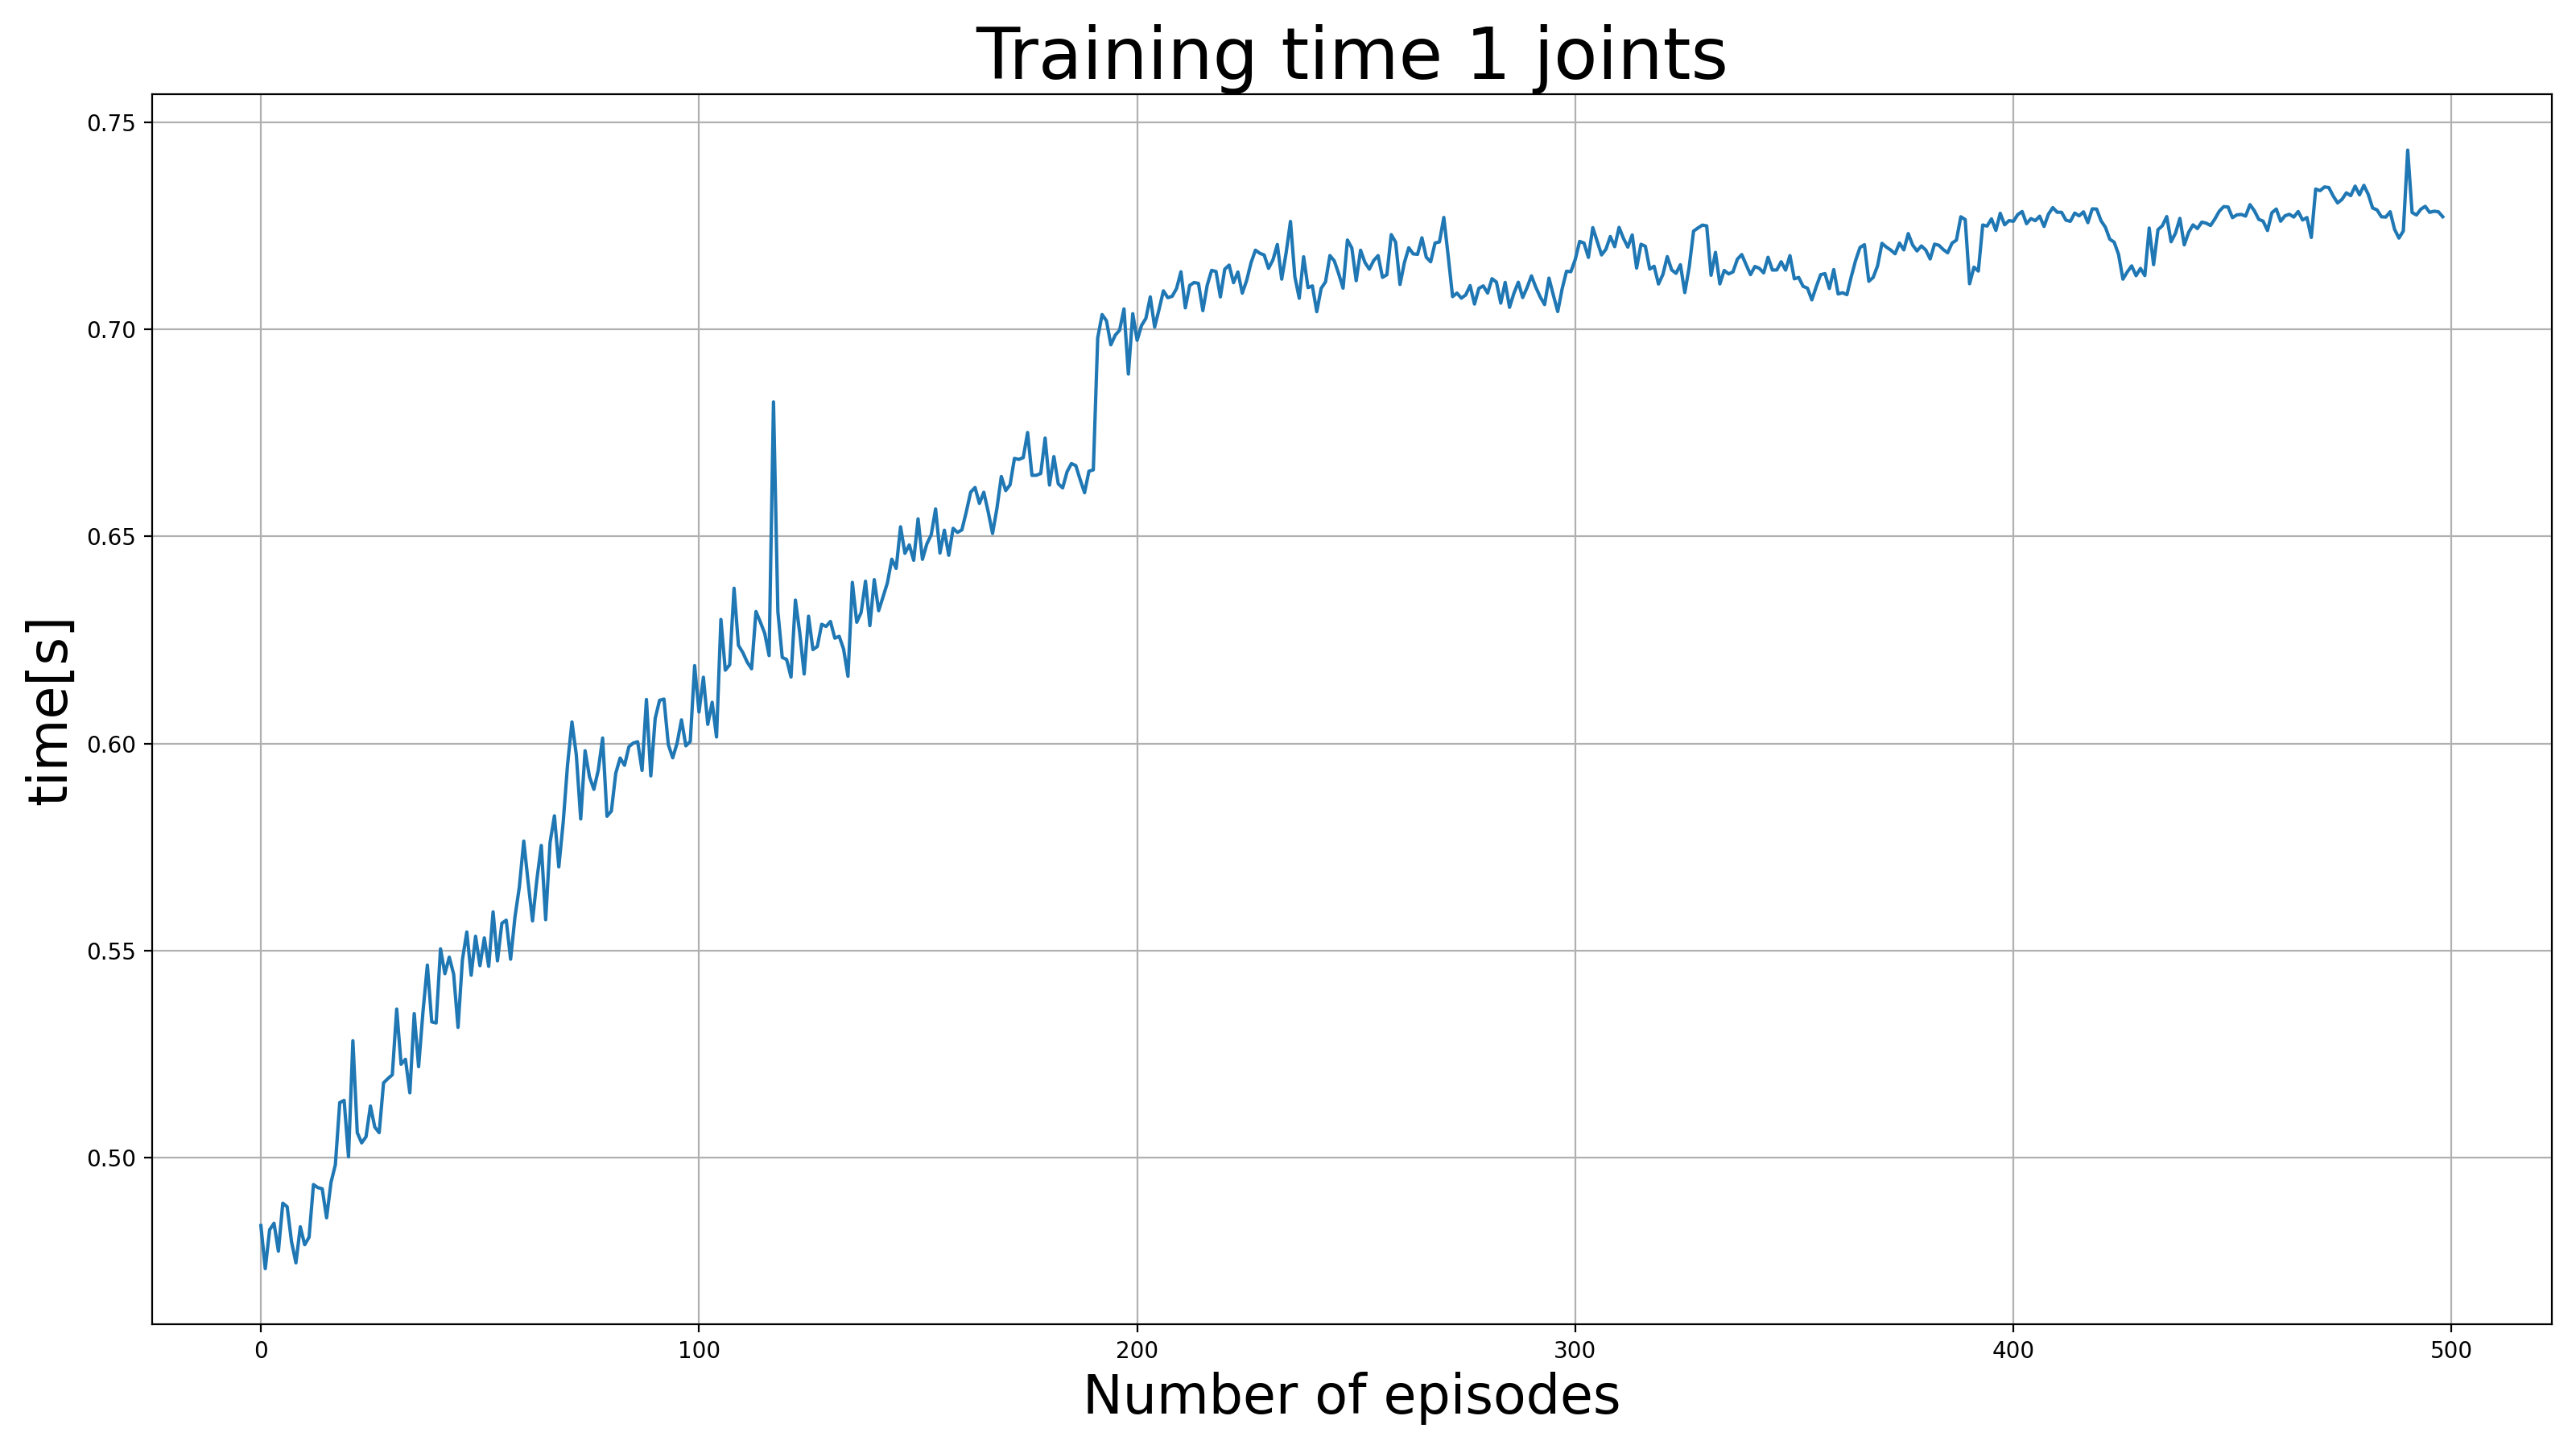
\includegraphics[width=8.5cm]{"../Figures/training_time_over_epiodes_1J_500E_256EL.png"}
	\caption{Training time having 1 joints.}
\end{figure}

Following are the results given by the testing phase.
\label{fig:Test_1_random_pos}
\begin{figure}[H]
	\centering
	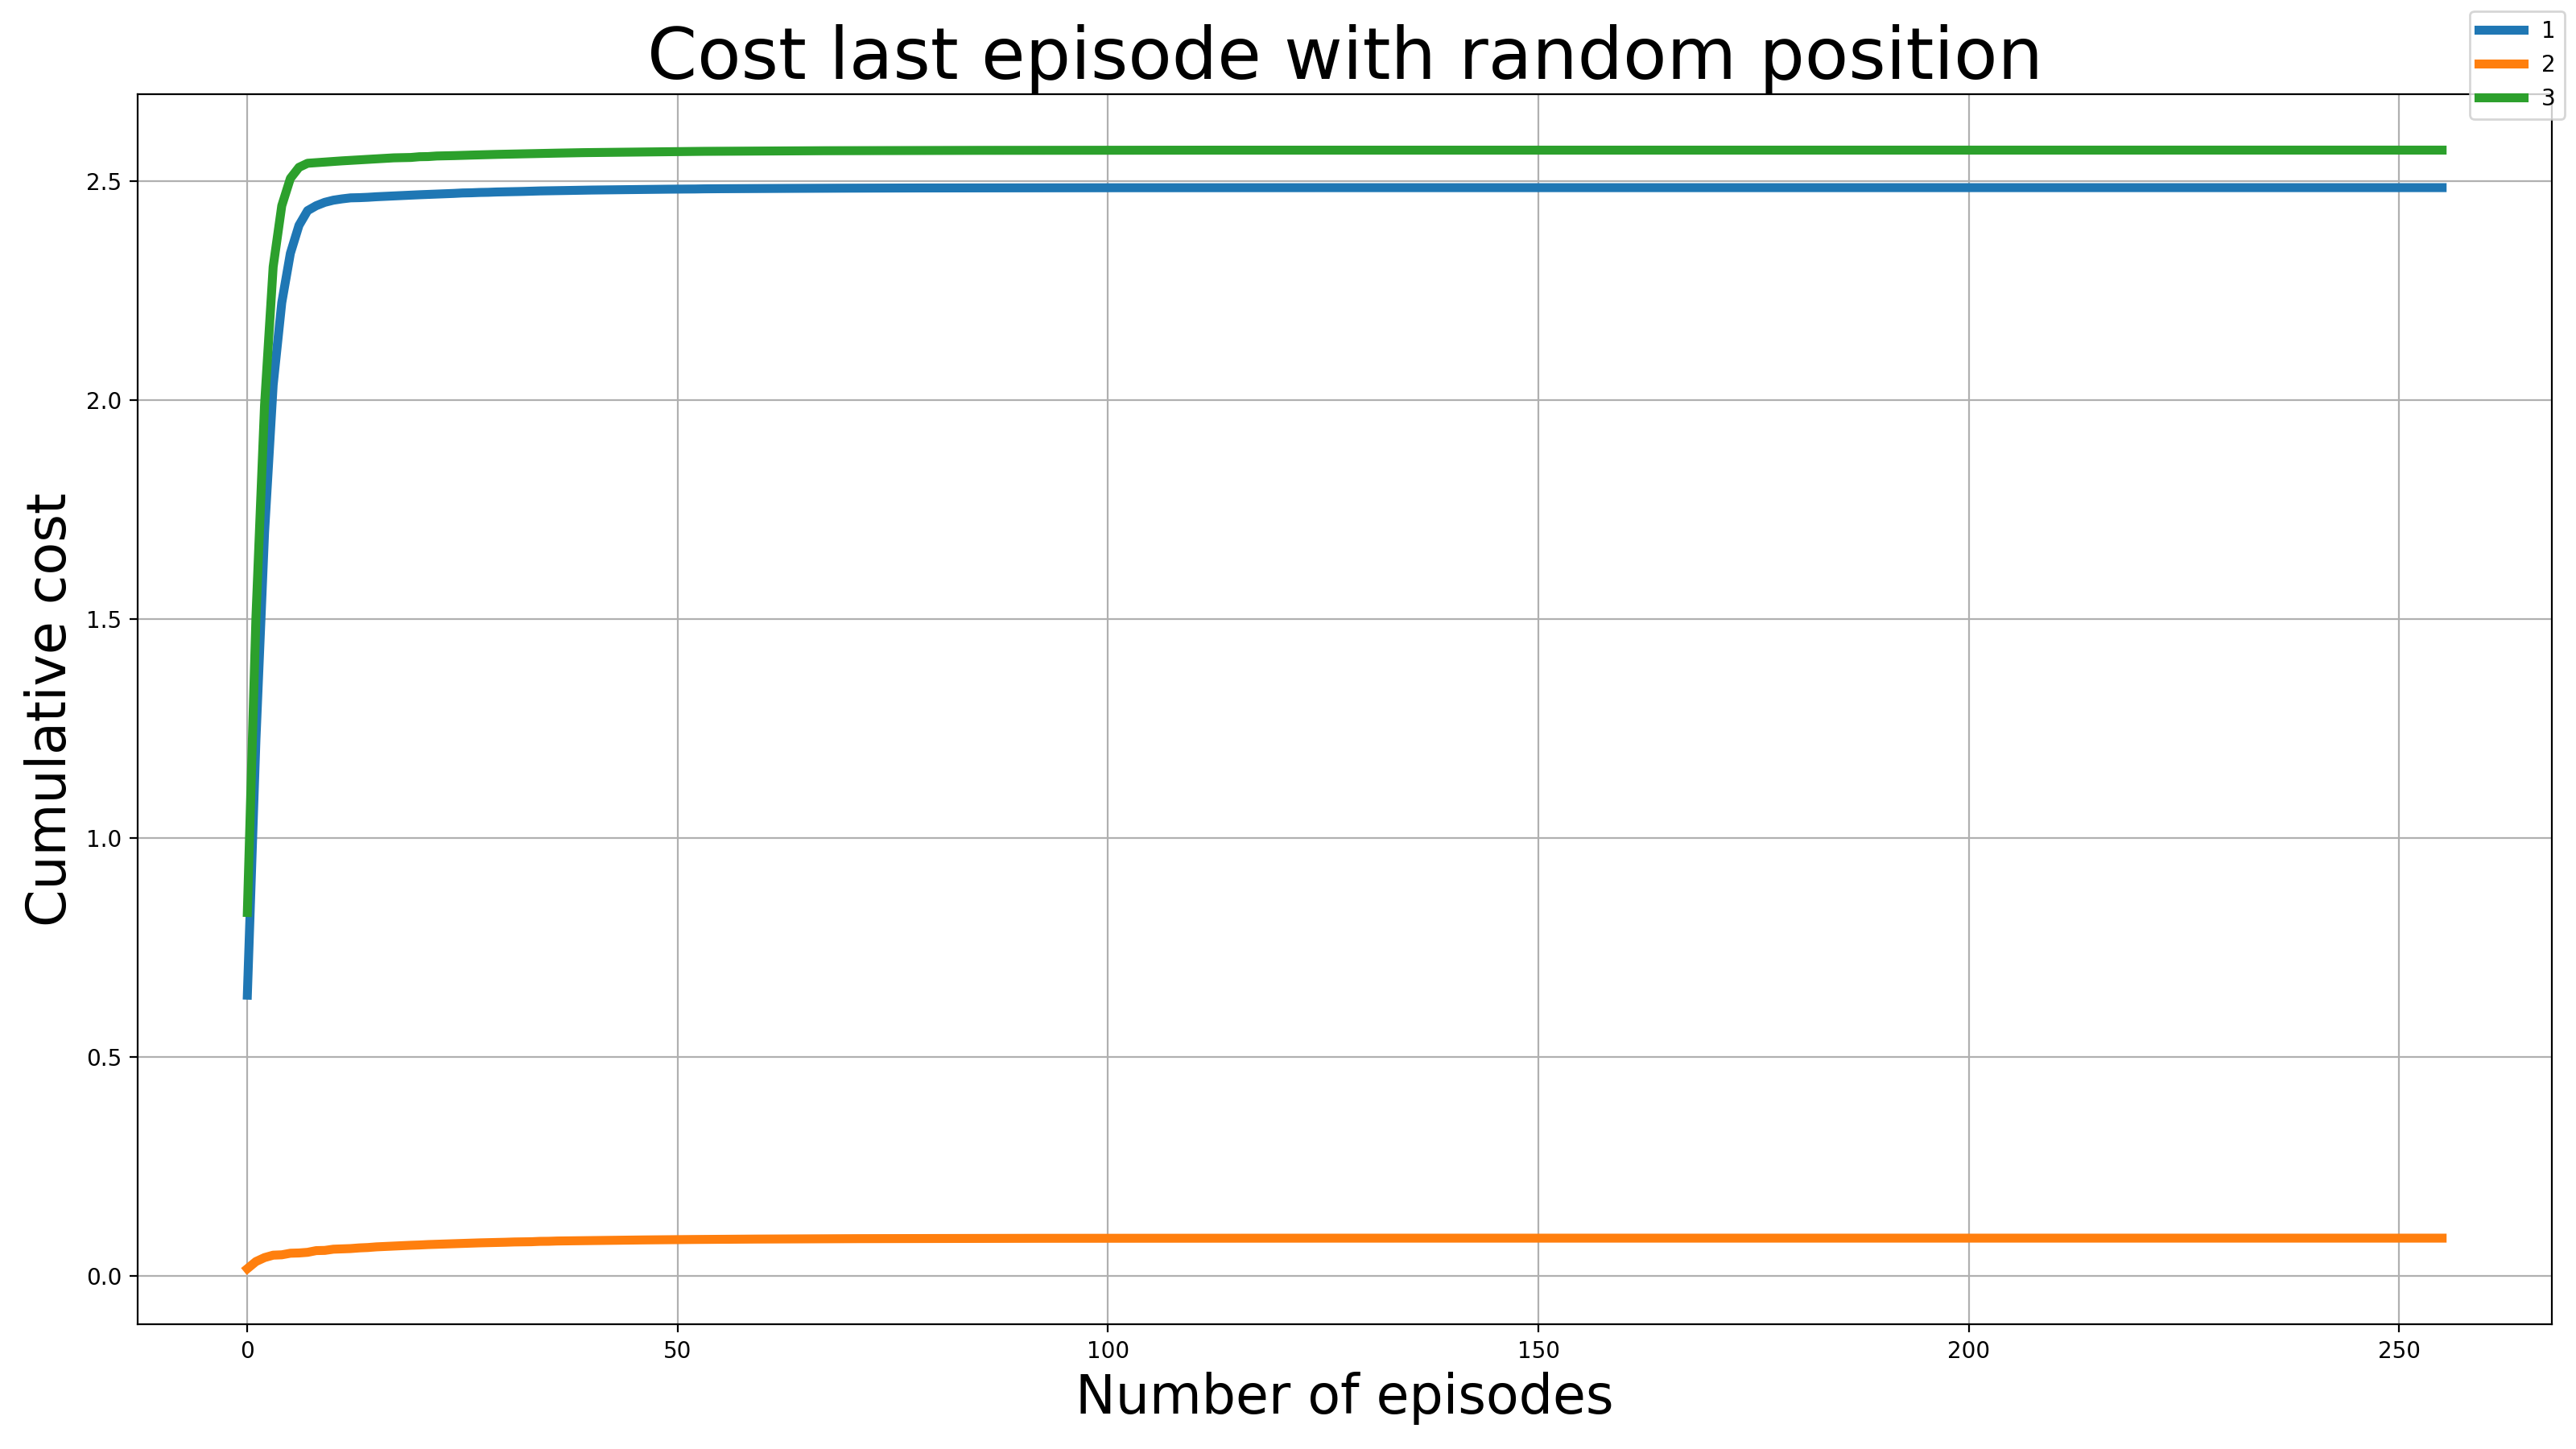
\includegraphics[width=8.5cm]{"../Figures/loss_last_ep_random_positions_1J_500E_256EL.png"}
	\caption{Total cost over the test episodes for the robot starting
			 from random positions.}
\end{figure}
\vspace{-1cm}
\label{fig:Test_1_down_pos}
\begin{figure}[H]
	\centering
	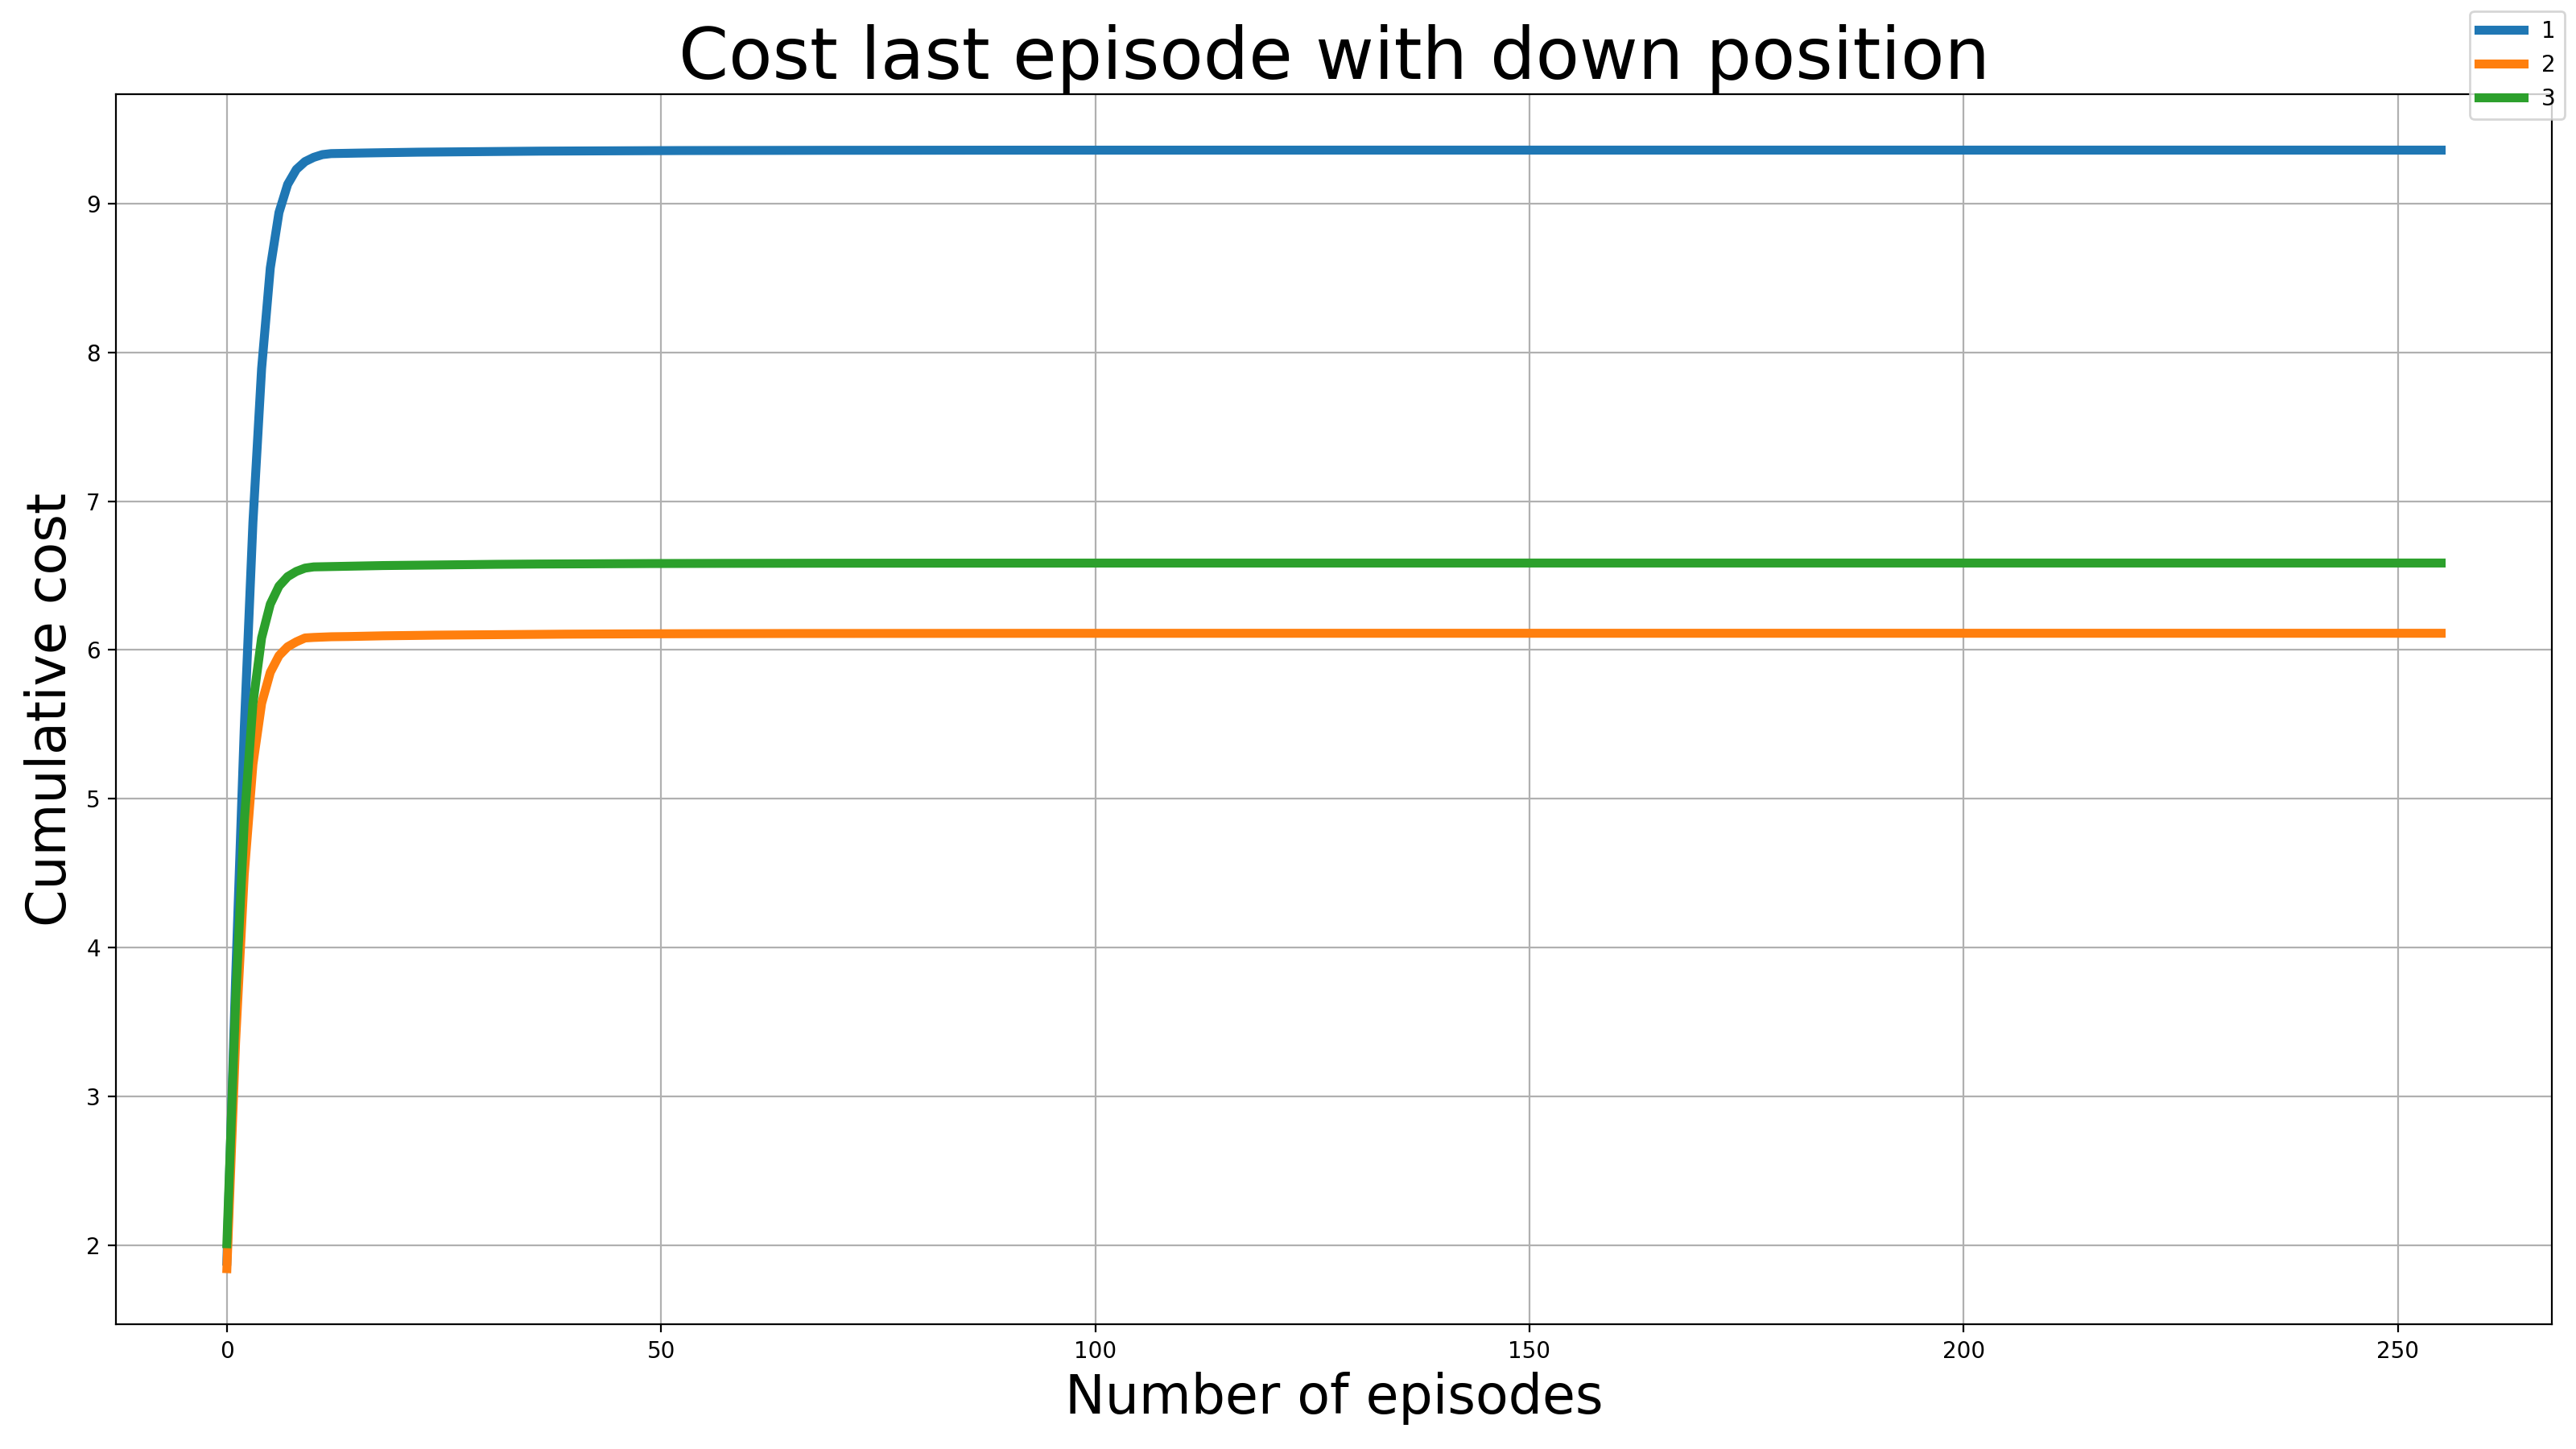
\includegraphics[width=8.5cm]{"../Figures/loss_last_ep_down_positions_1J_500E_256EL.png"}
	\caption{Total cost over the test episodes for the robot starting
			 from the down position.}
\end{figure}
\vspace{-1cm}
\label{fig:Test_1_best_random_pos}
\begin{figure}[H]
	\centering
	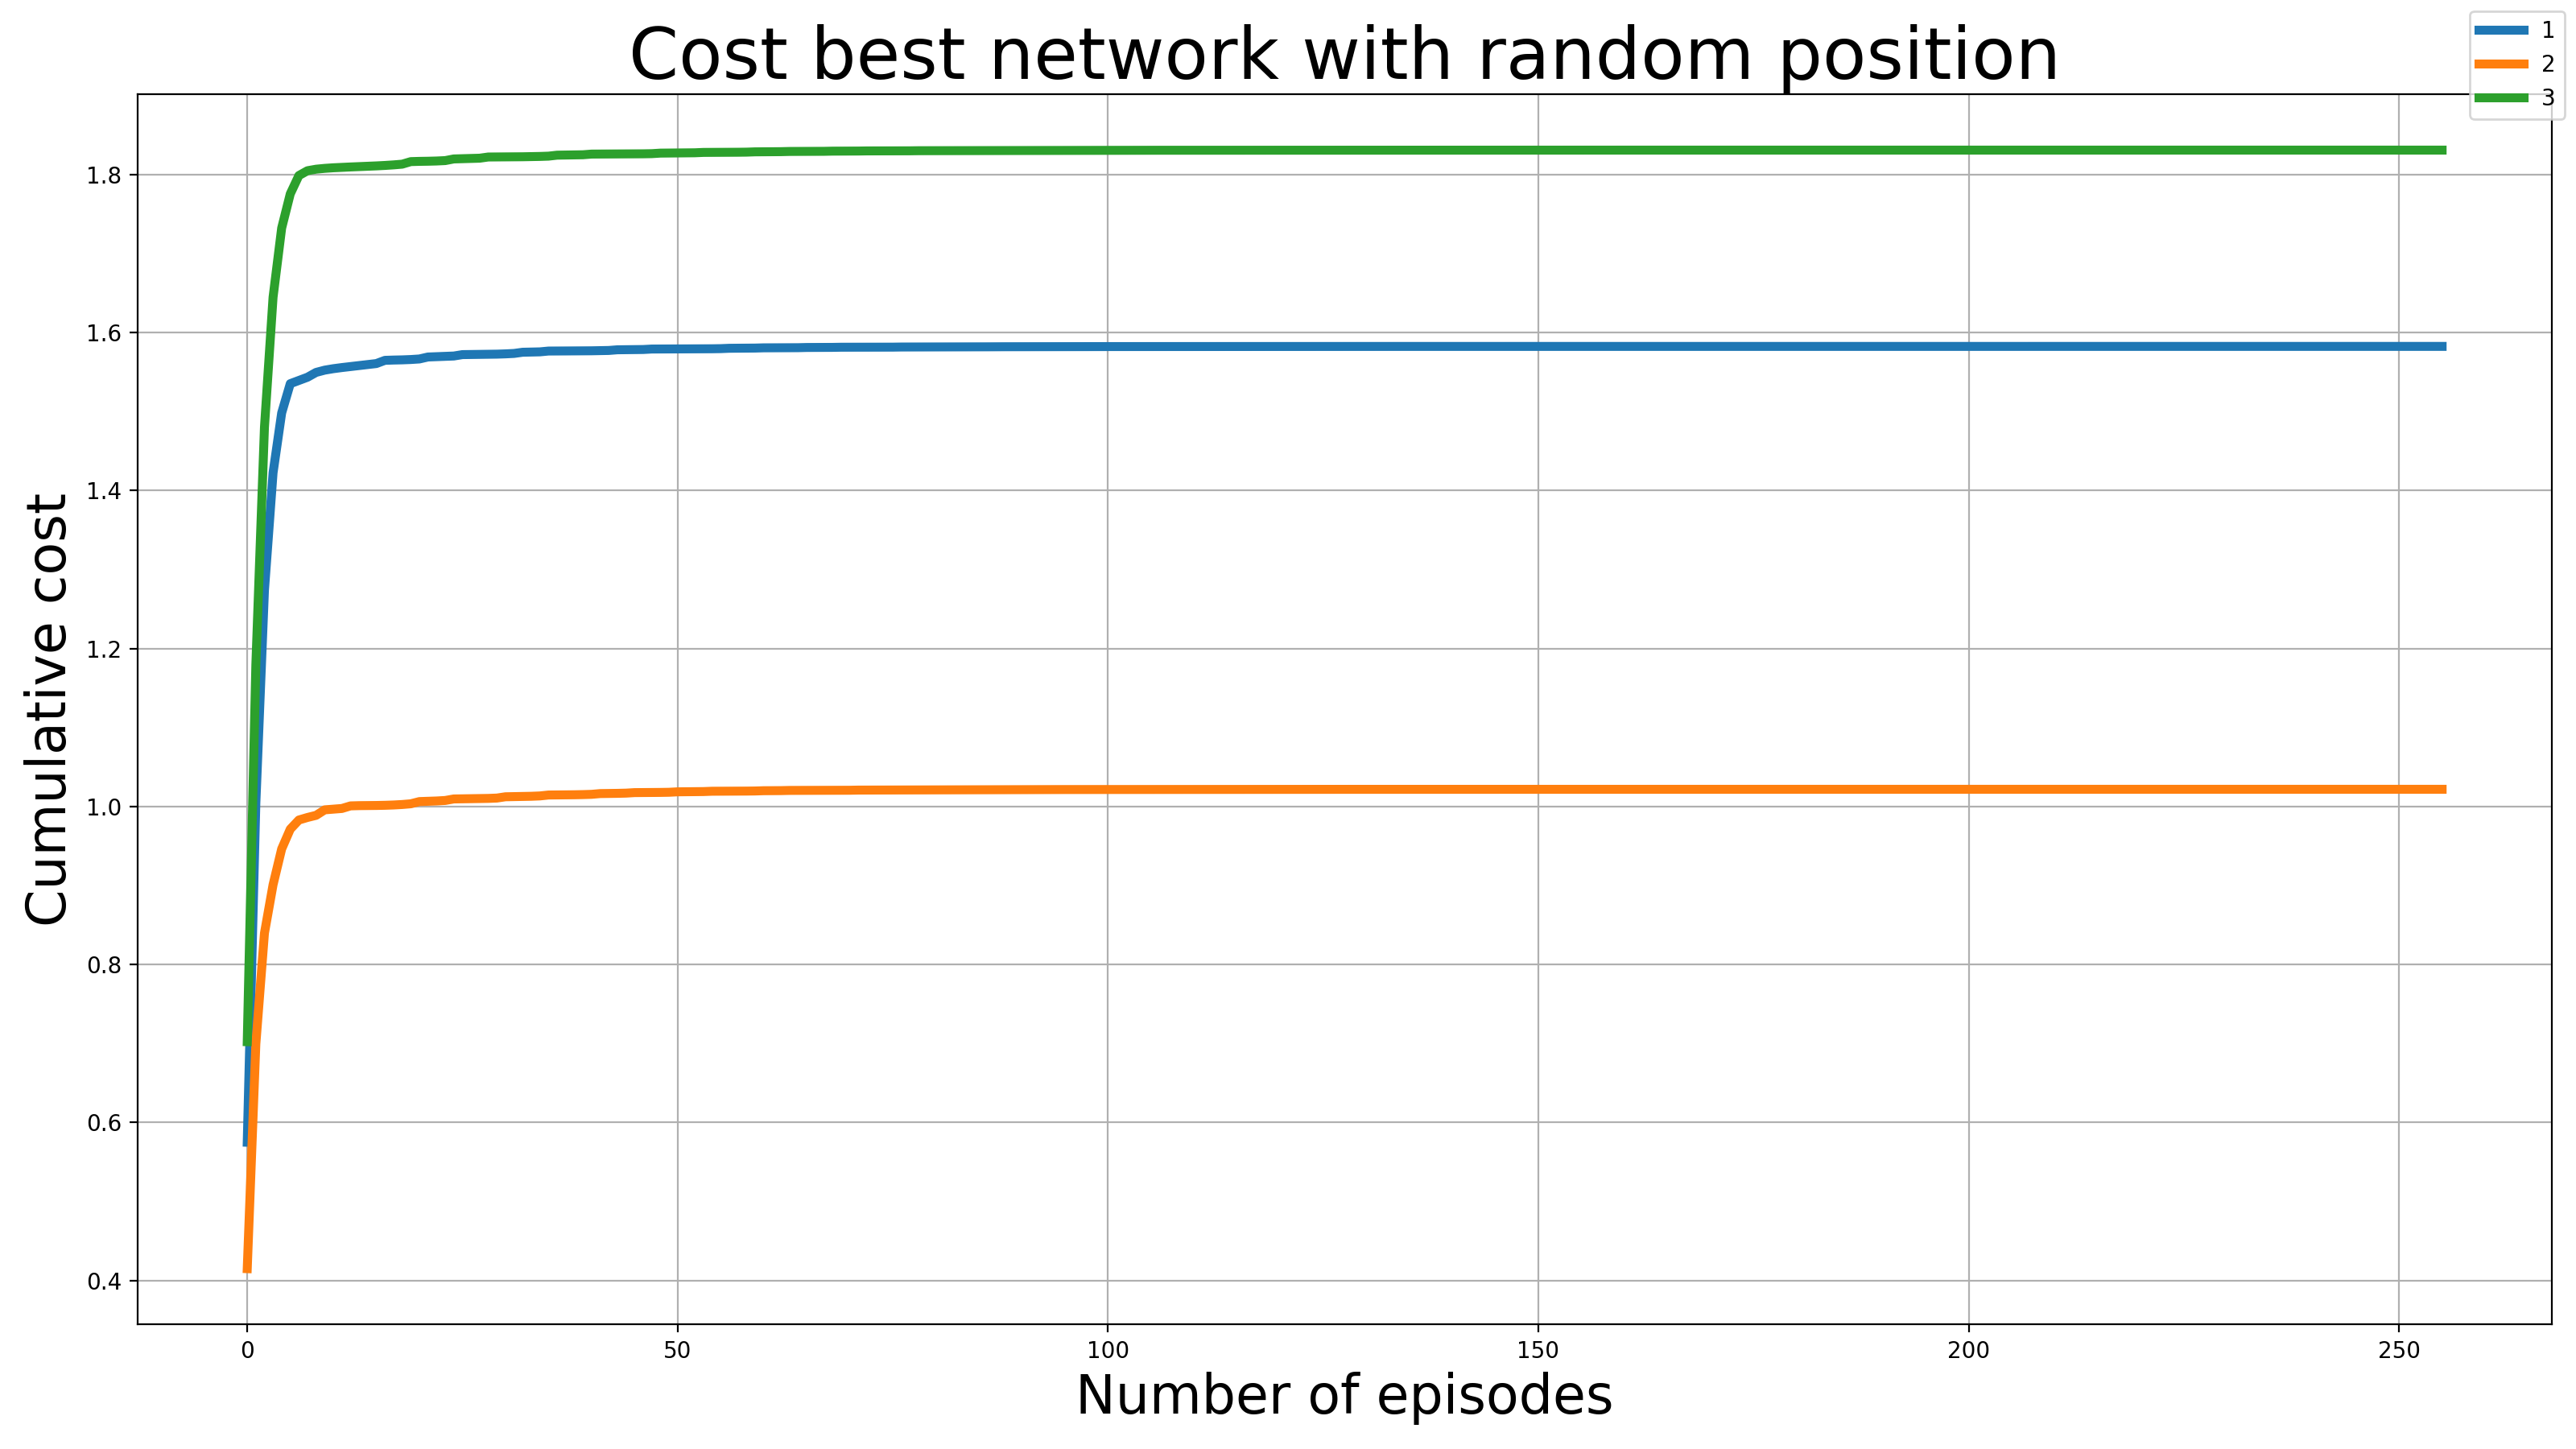
\includegraphics[width=8.5cm]{"../Figures/loss_best_net_random_positions_1J_500E_256EL.png"}
	\caption{Total cost over the test episodes for the robot starting from
			 random positions using the best performing network.}
\end{figure}
\vspace{-1cm}
\label{fig:Test_1_best_down_pos}
\begin{figure}[H]
	\centering
	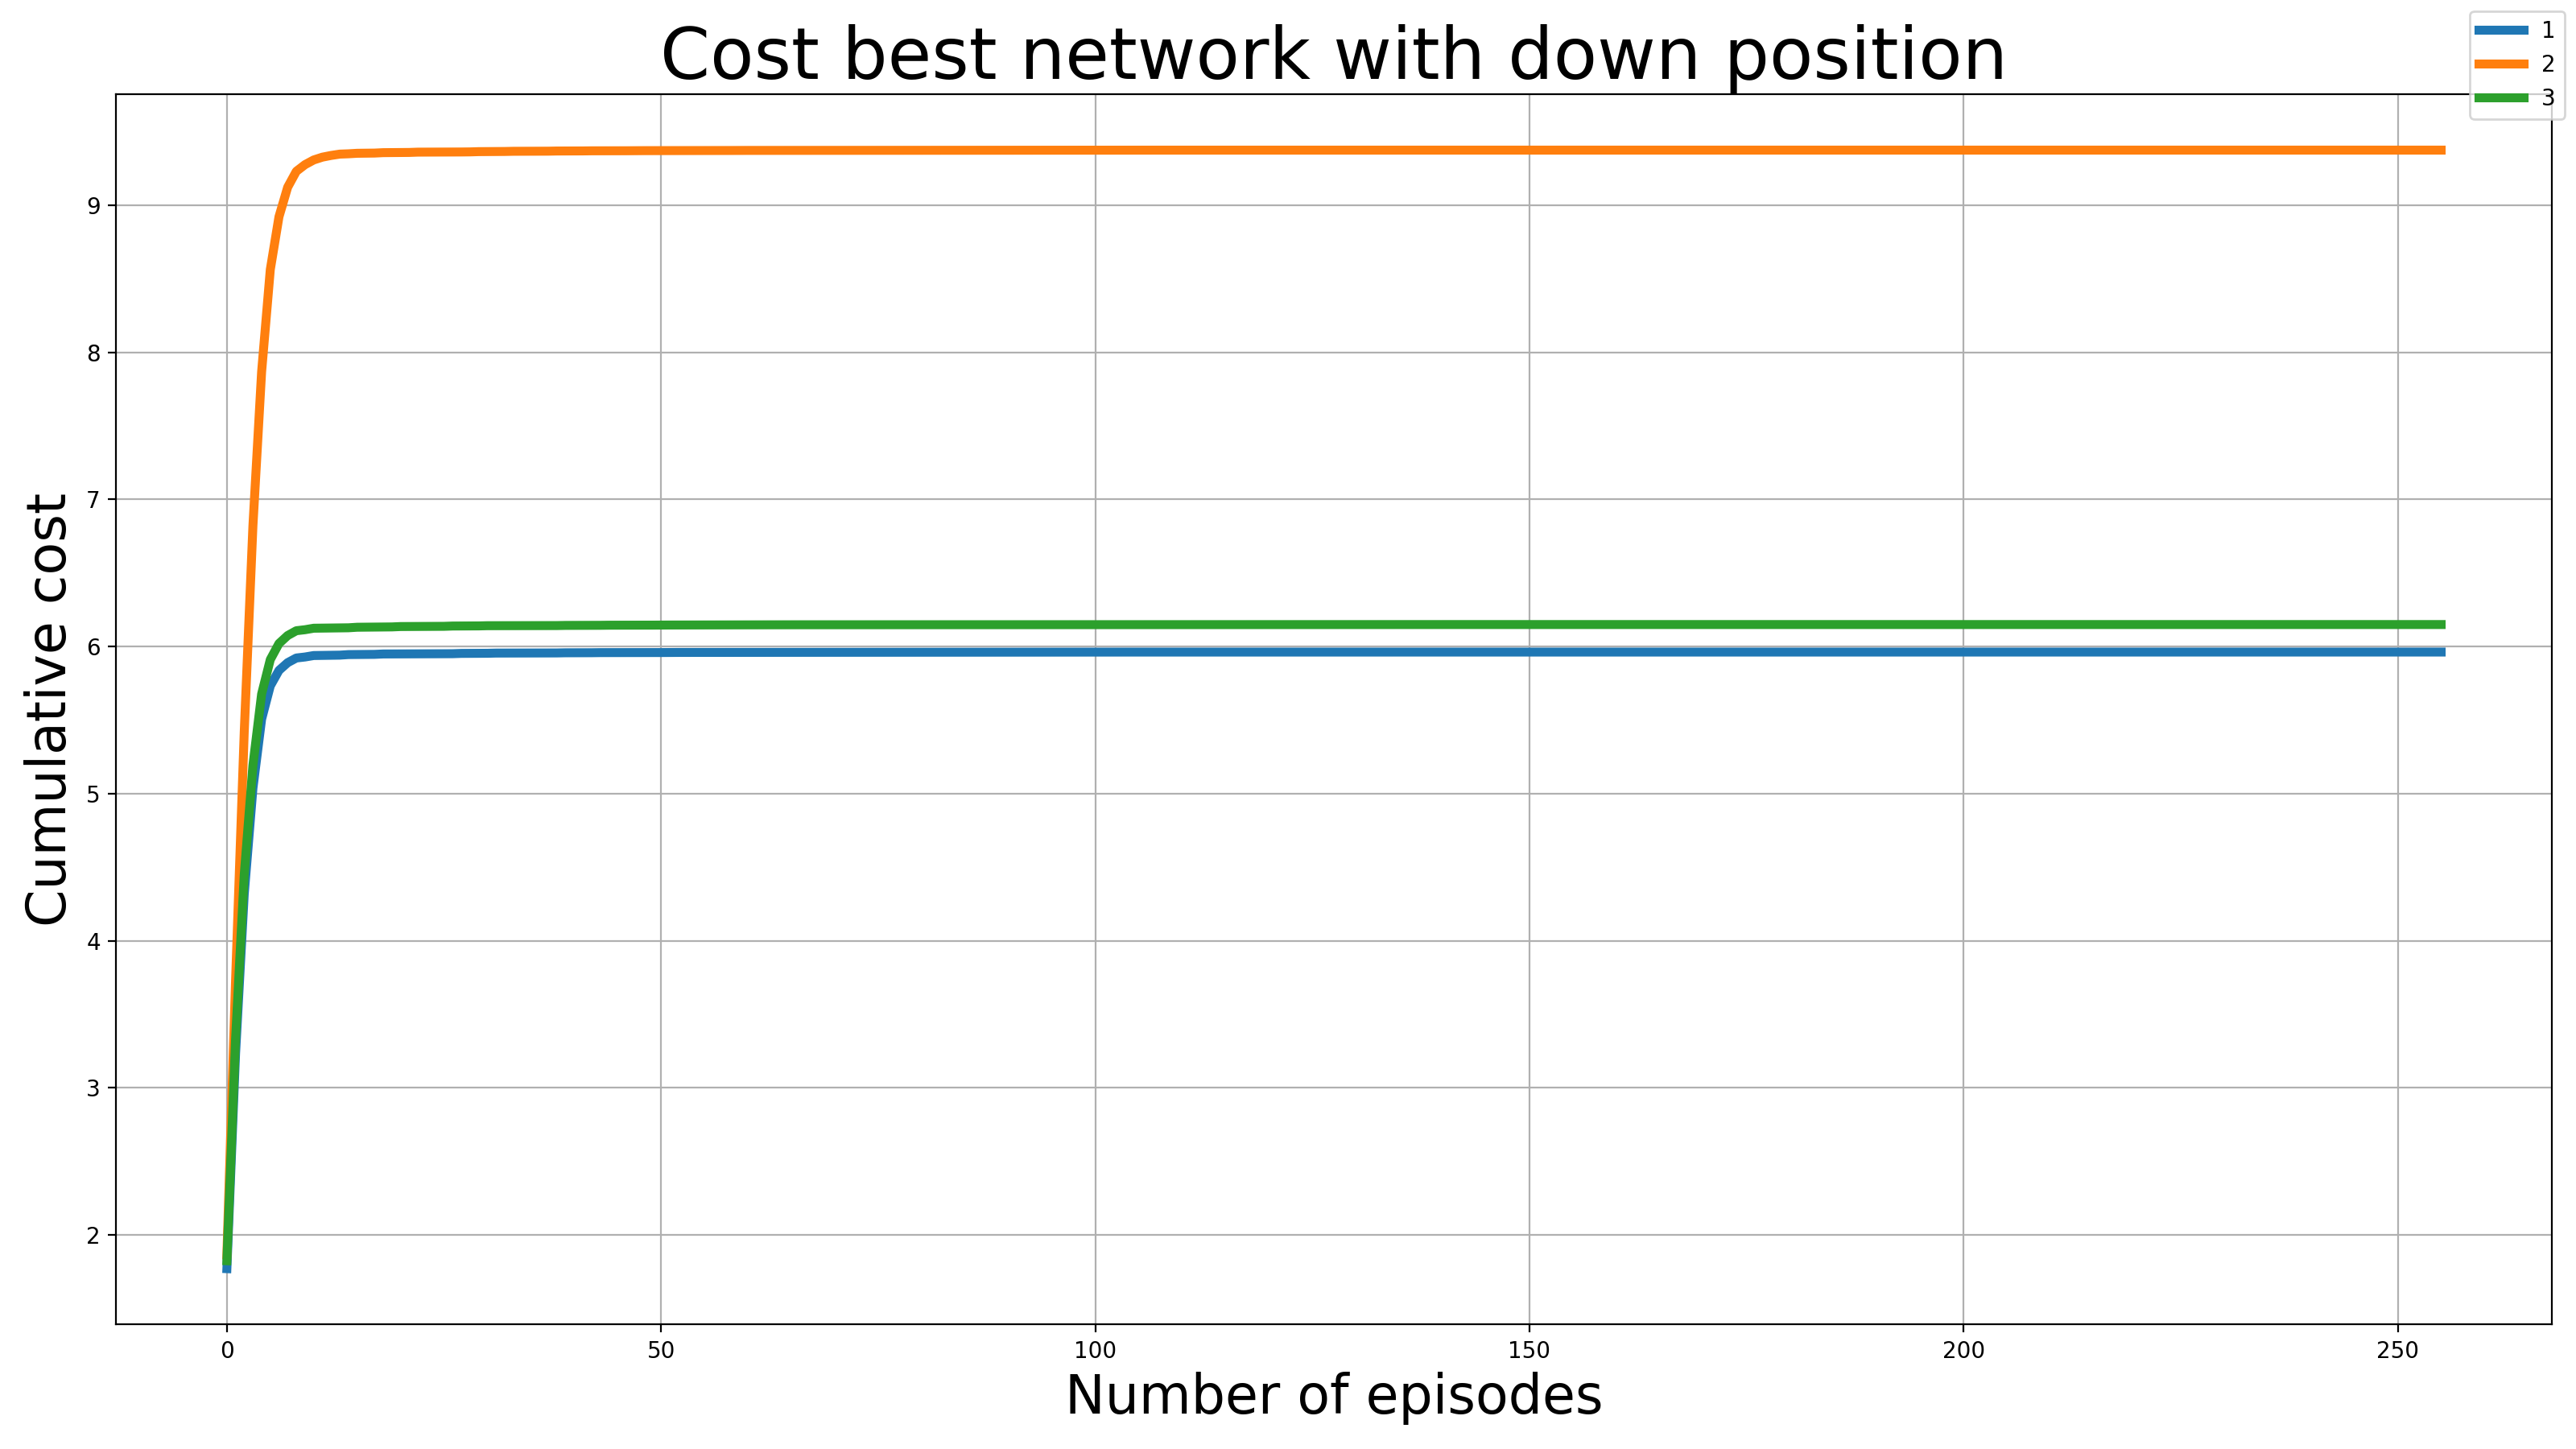
\includegraphics[width=8.5cm]{"../Figures/loss_best_net_down_positions_1J_500E_256EL.png"}
	\caption{Total cost over the test episodes for the robot starting from
			 down positions using the best performing network.}
\end{figure}

\subsection{2 joints}
Following are shown the results in case the robot has 2 joints.

\label{fig:TrainLoss2}
\begin{figure}[H]
	\centering
	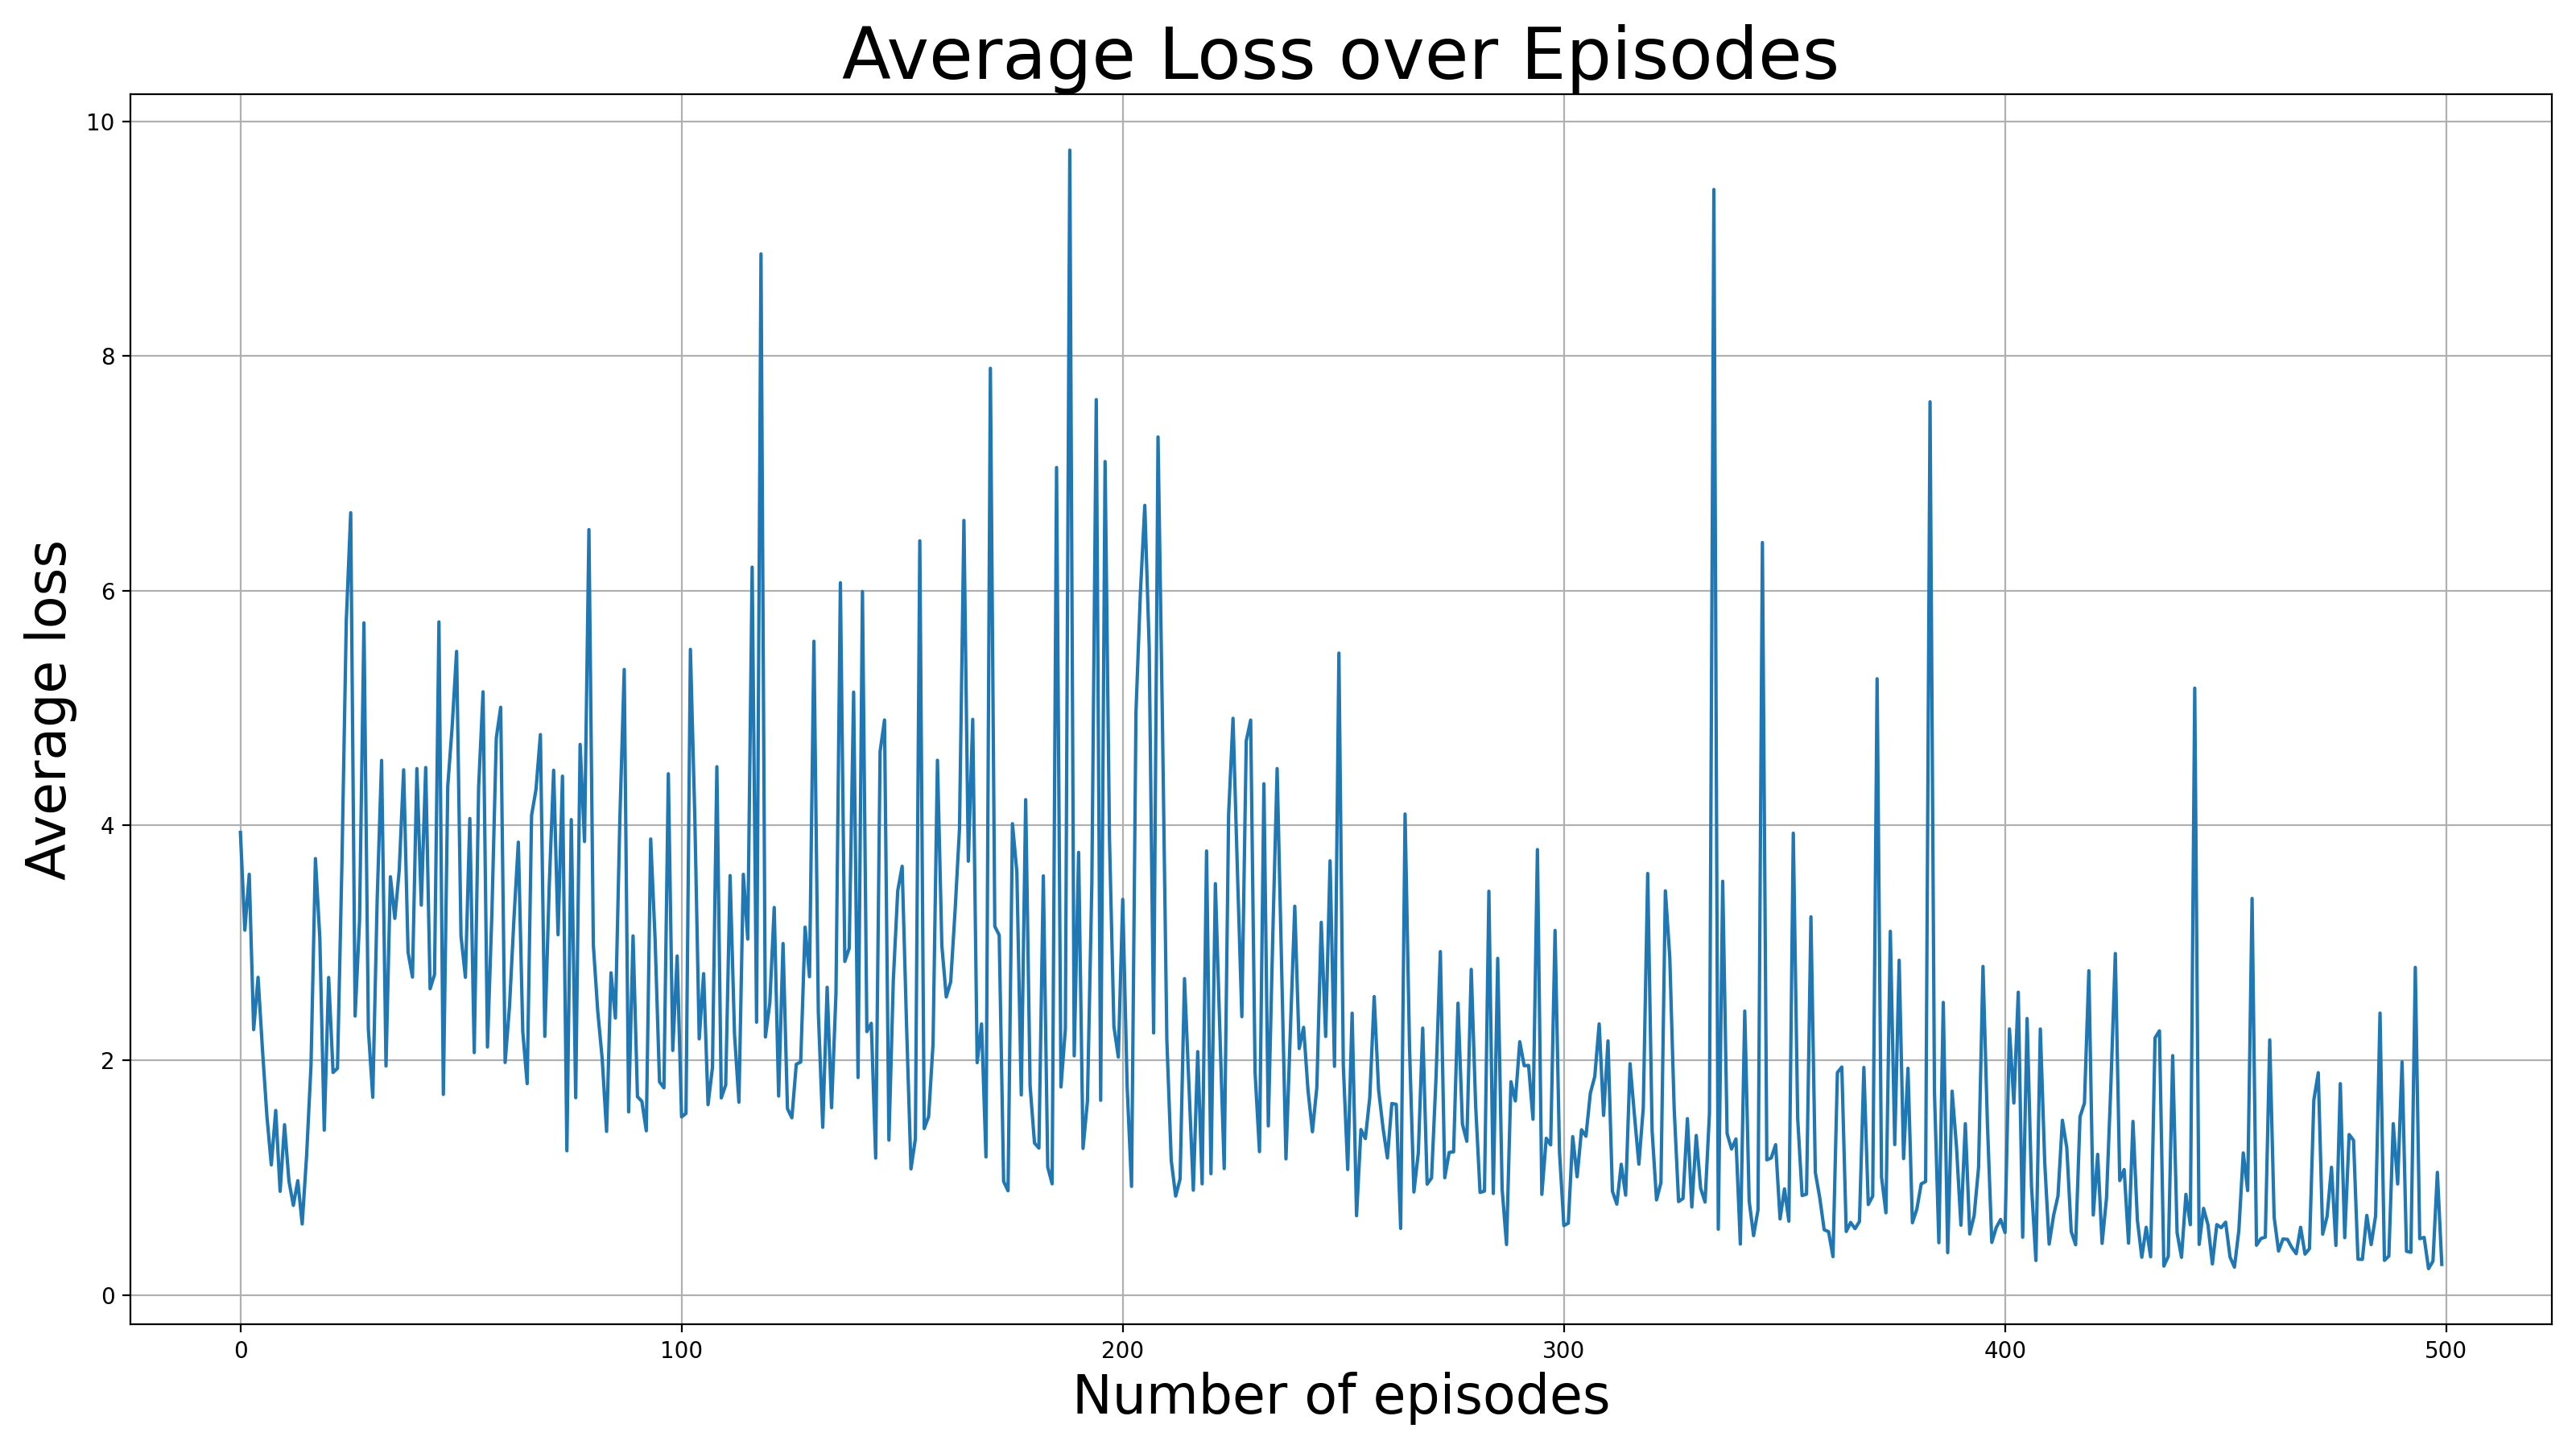
\includegraphics[width=8.5cm]{"../Figures/average_loss_over_epiodes_2J_500E_256EL.png"}
	\caption{Training loss having 2 joints.}
\end{figure}
\vspace{-0.5cm}
\label{fig:TrainTime2}
\begin{figure}[H]
	\centering
	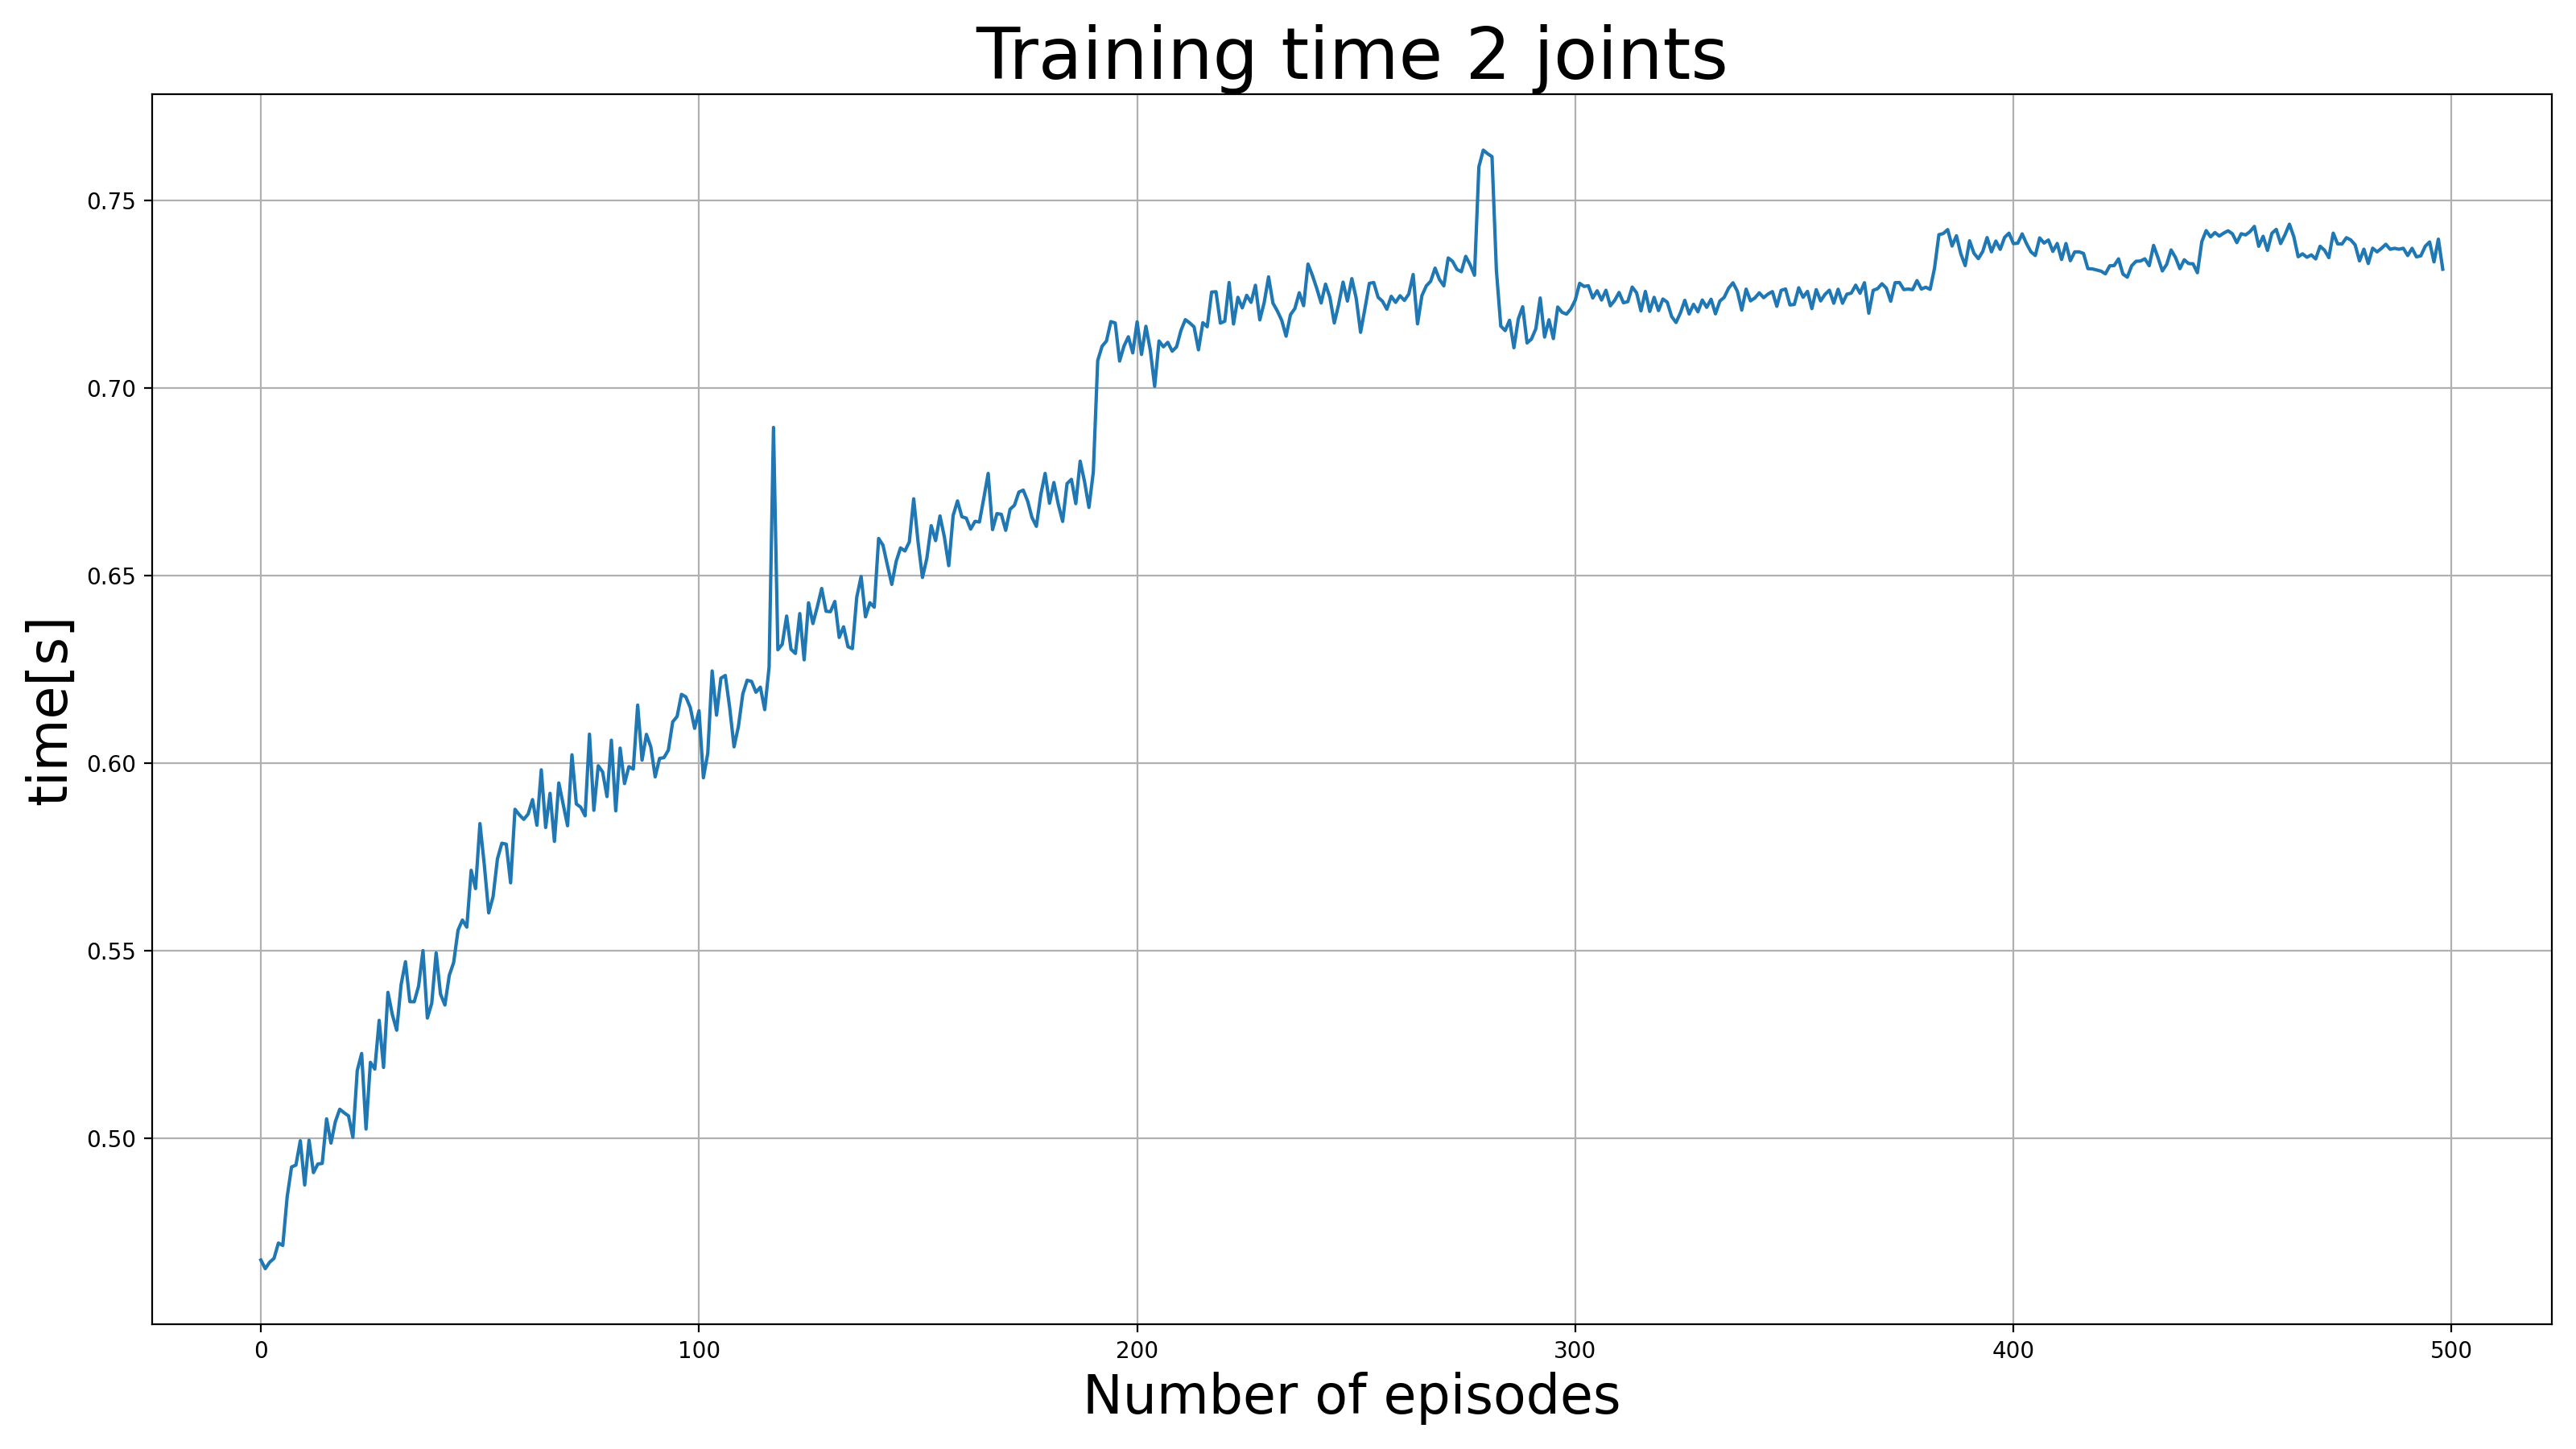
\includegraphics[width=8.5cm]{"../Figures/training_time_over_epiodes_2J_500E_256EL.png"}
	\caption{Training time having 2 joints.}
\end{figure}
\vspace{-0.5cm}
Following are the results given by the testing phase.
\label{fig:Test_2_random_pos}
\begin{figure}[H]
	\centering
	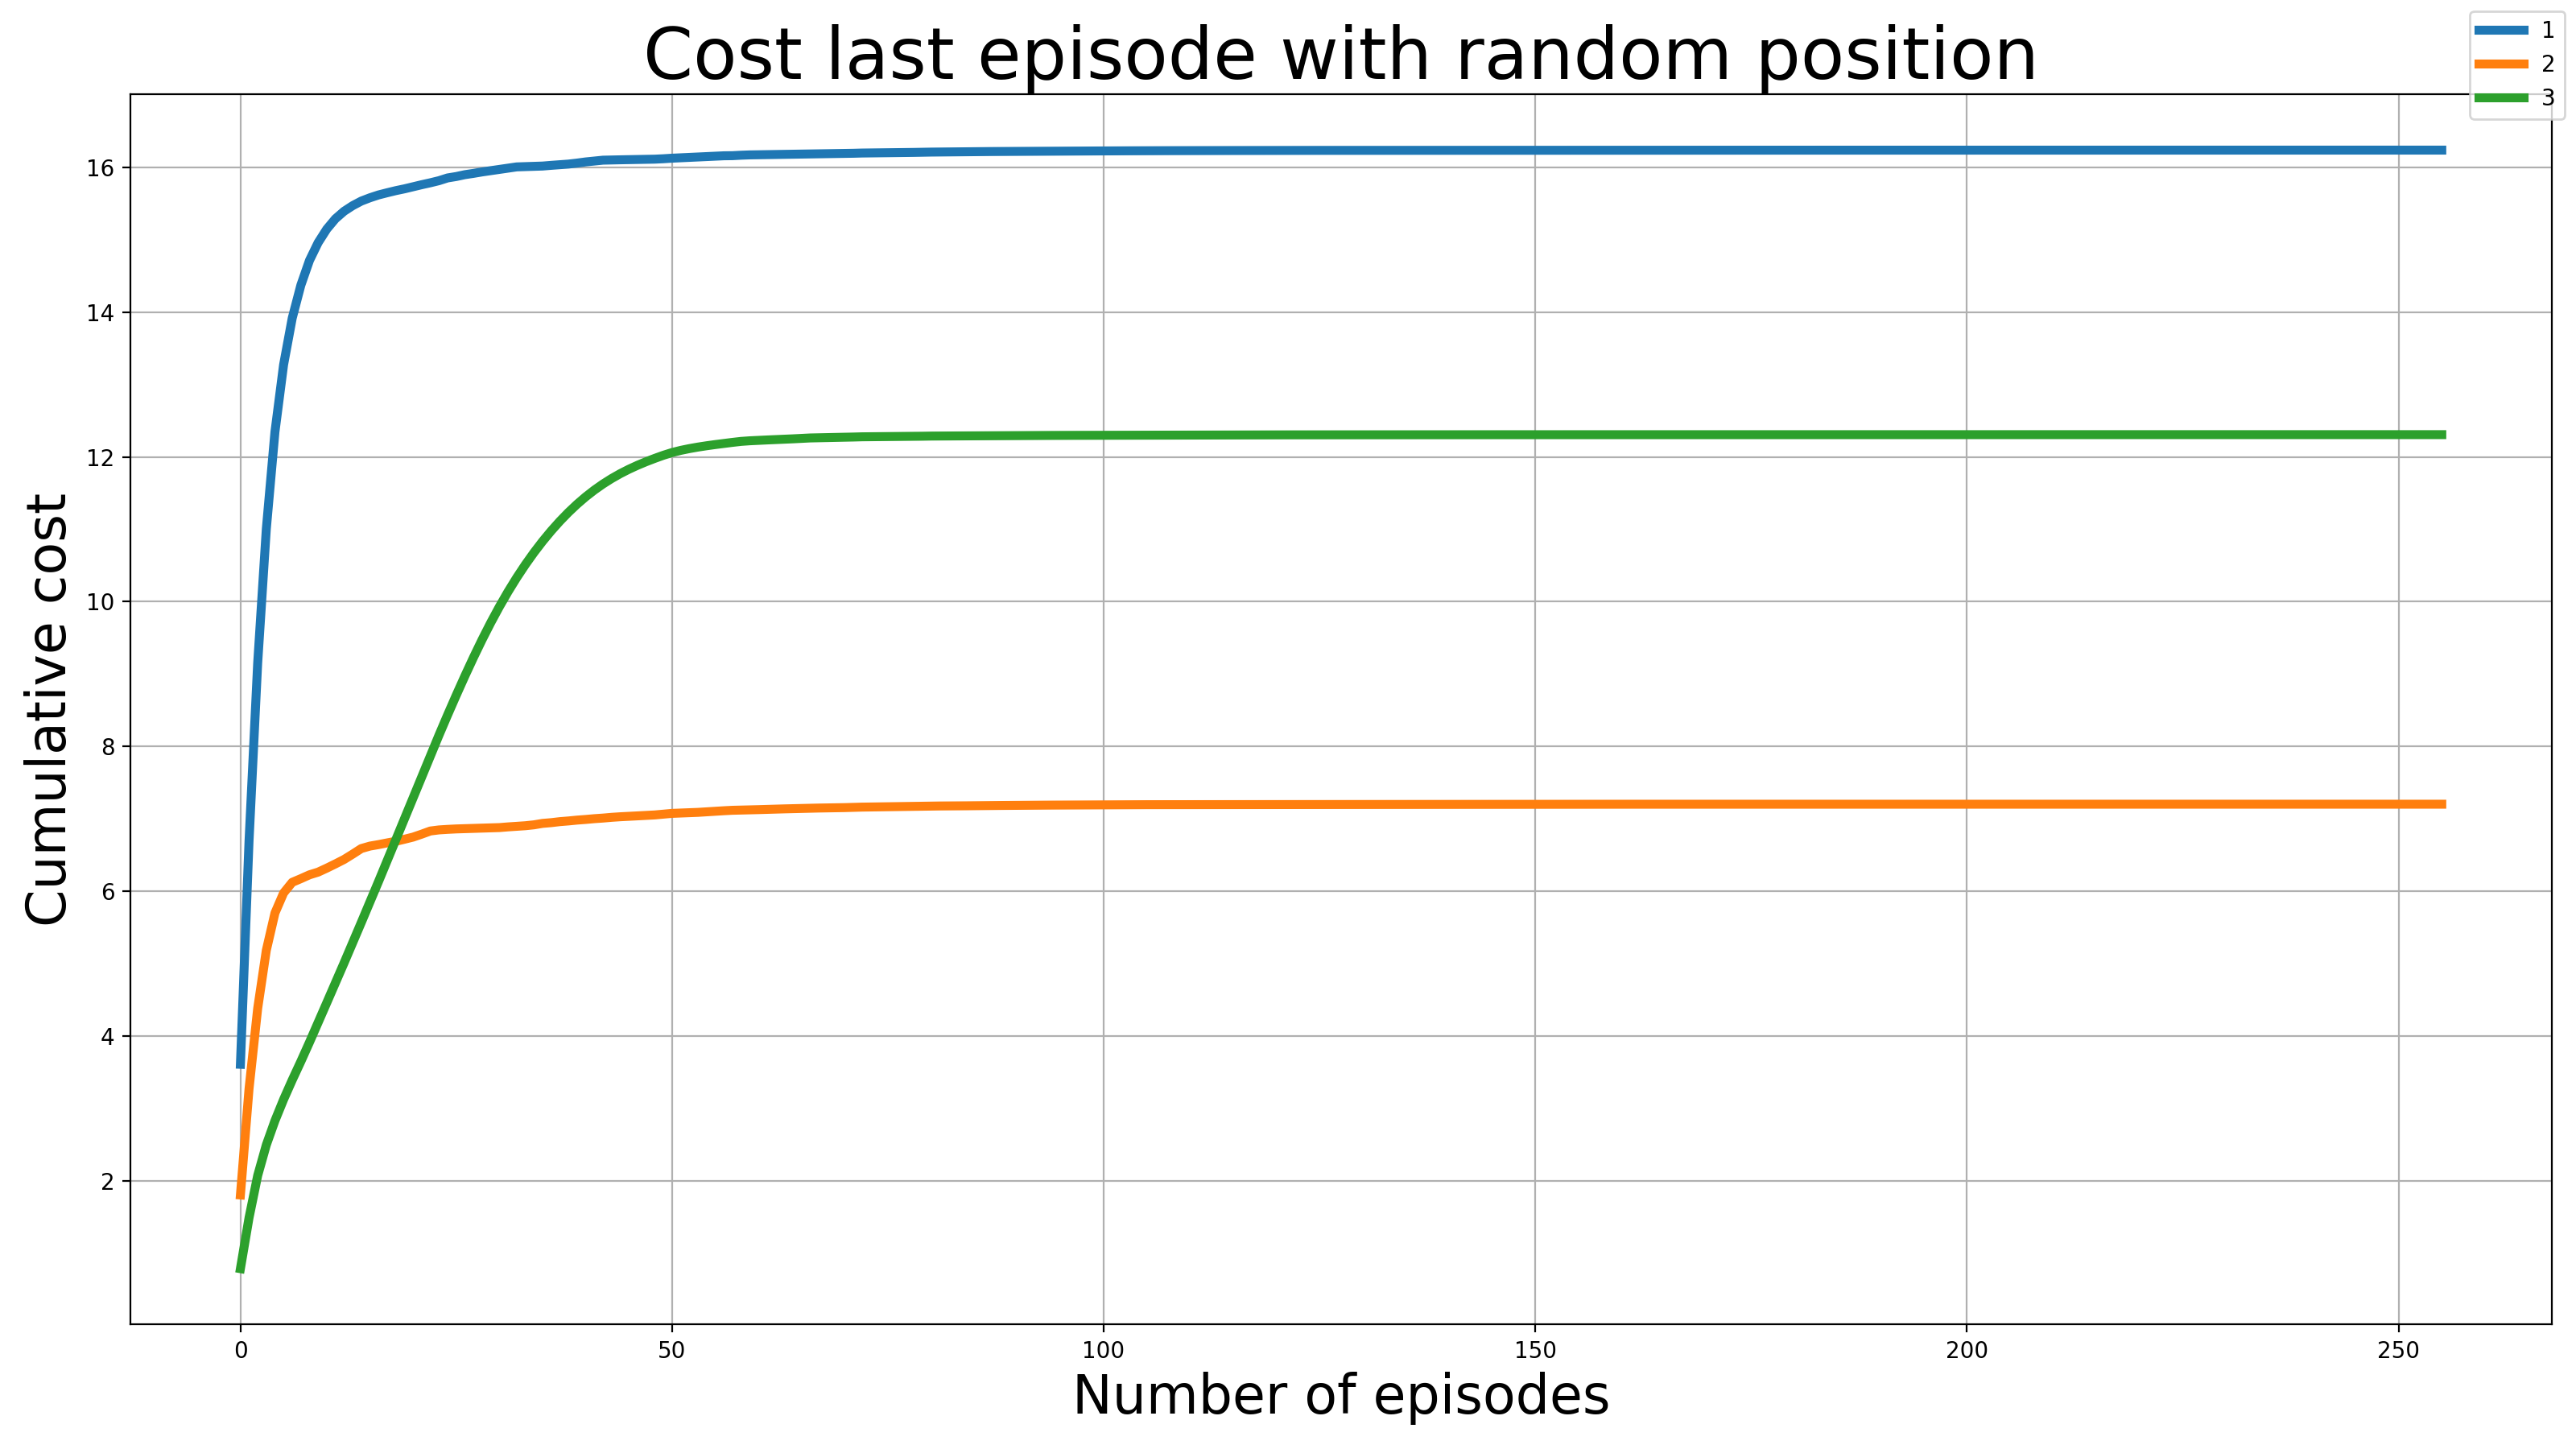
\includegraphics[width=8.5cm]{"../Figures/loss_last_ep_random_positions_2J_500E_256EL.png"}
	\caption{Total cost over the test episodes for the robot starting
			 from random positions.}
\end{figure}
\vspace{-0.5cm}
\label{fig:Test_2_down_pos}
\begin{figure}[H]
	\centering
	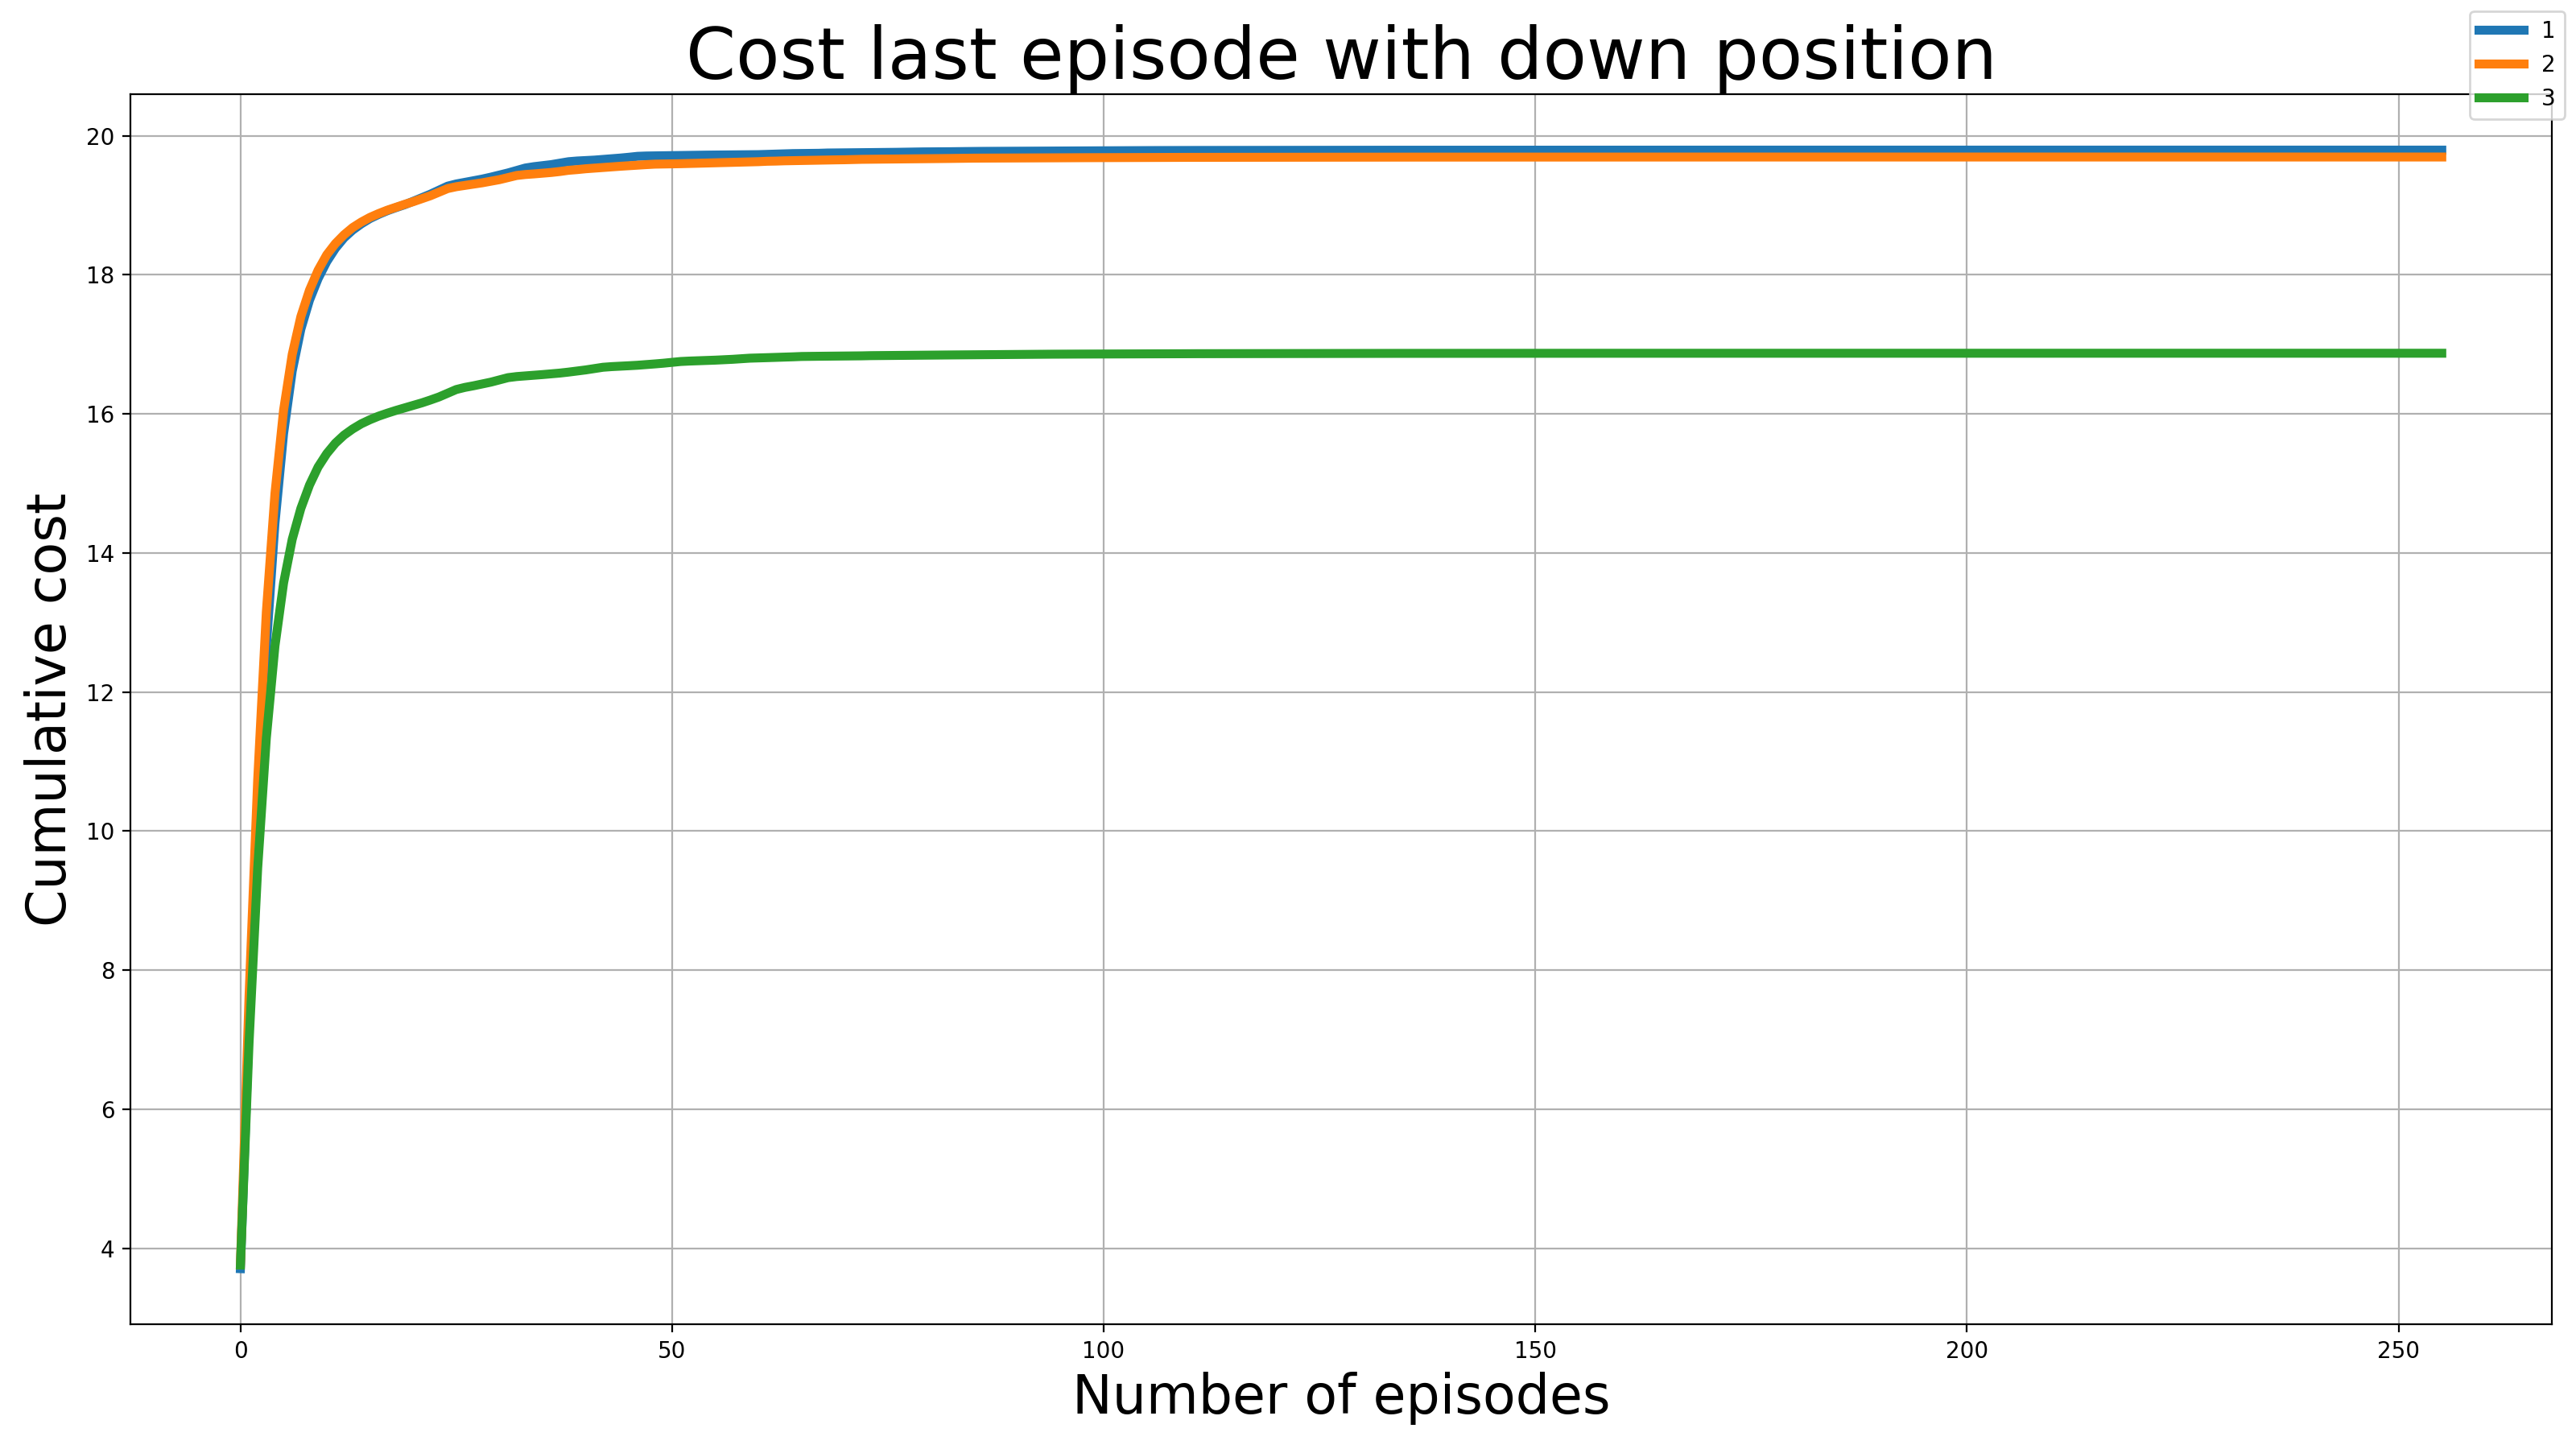
\includegraphics[width=8.5cm]{"../Figures/loss_last_ep_down_positions_2J_500E_256EL.png"}
	\caption{Total cost over the test episodes for the robot starting
			 from the down position.}
\end{figure}
\vspace{-0.5cm}
\label{fig:Test_2_best_random_pos}
\begin{figure}[H]
	\centering
	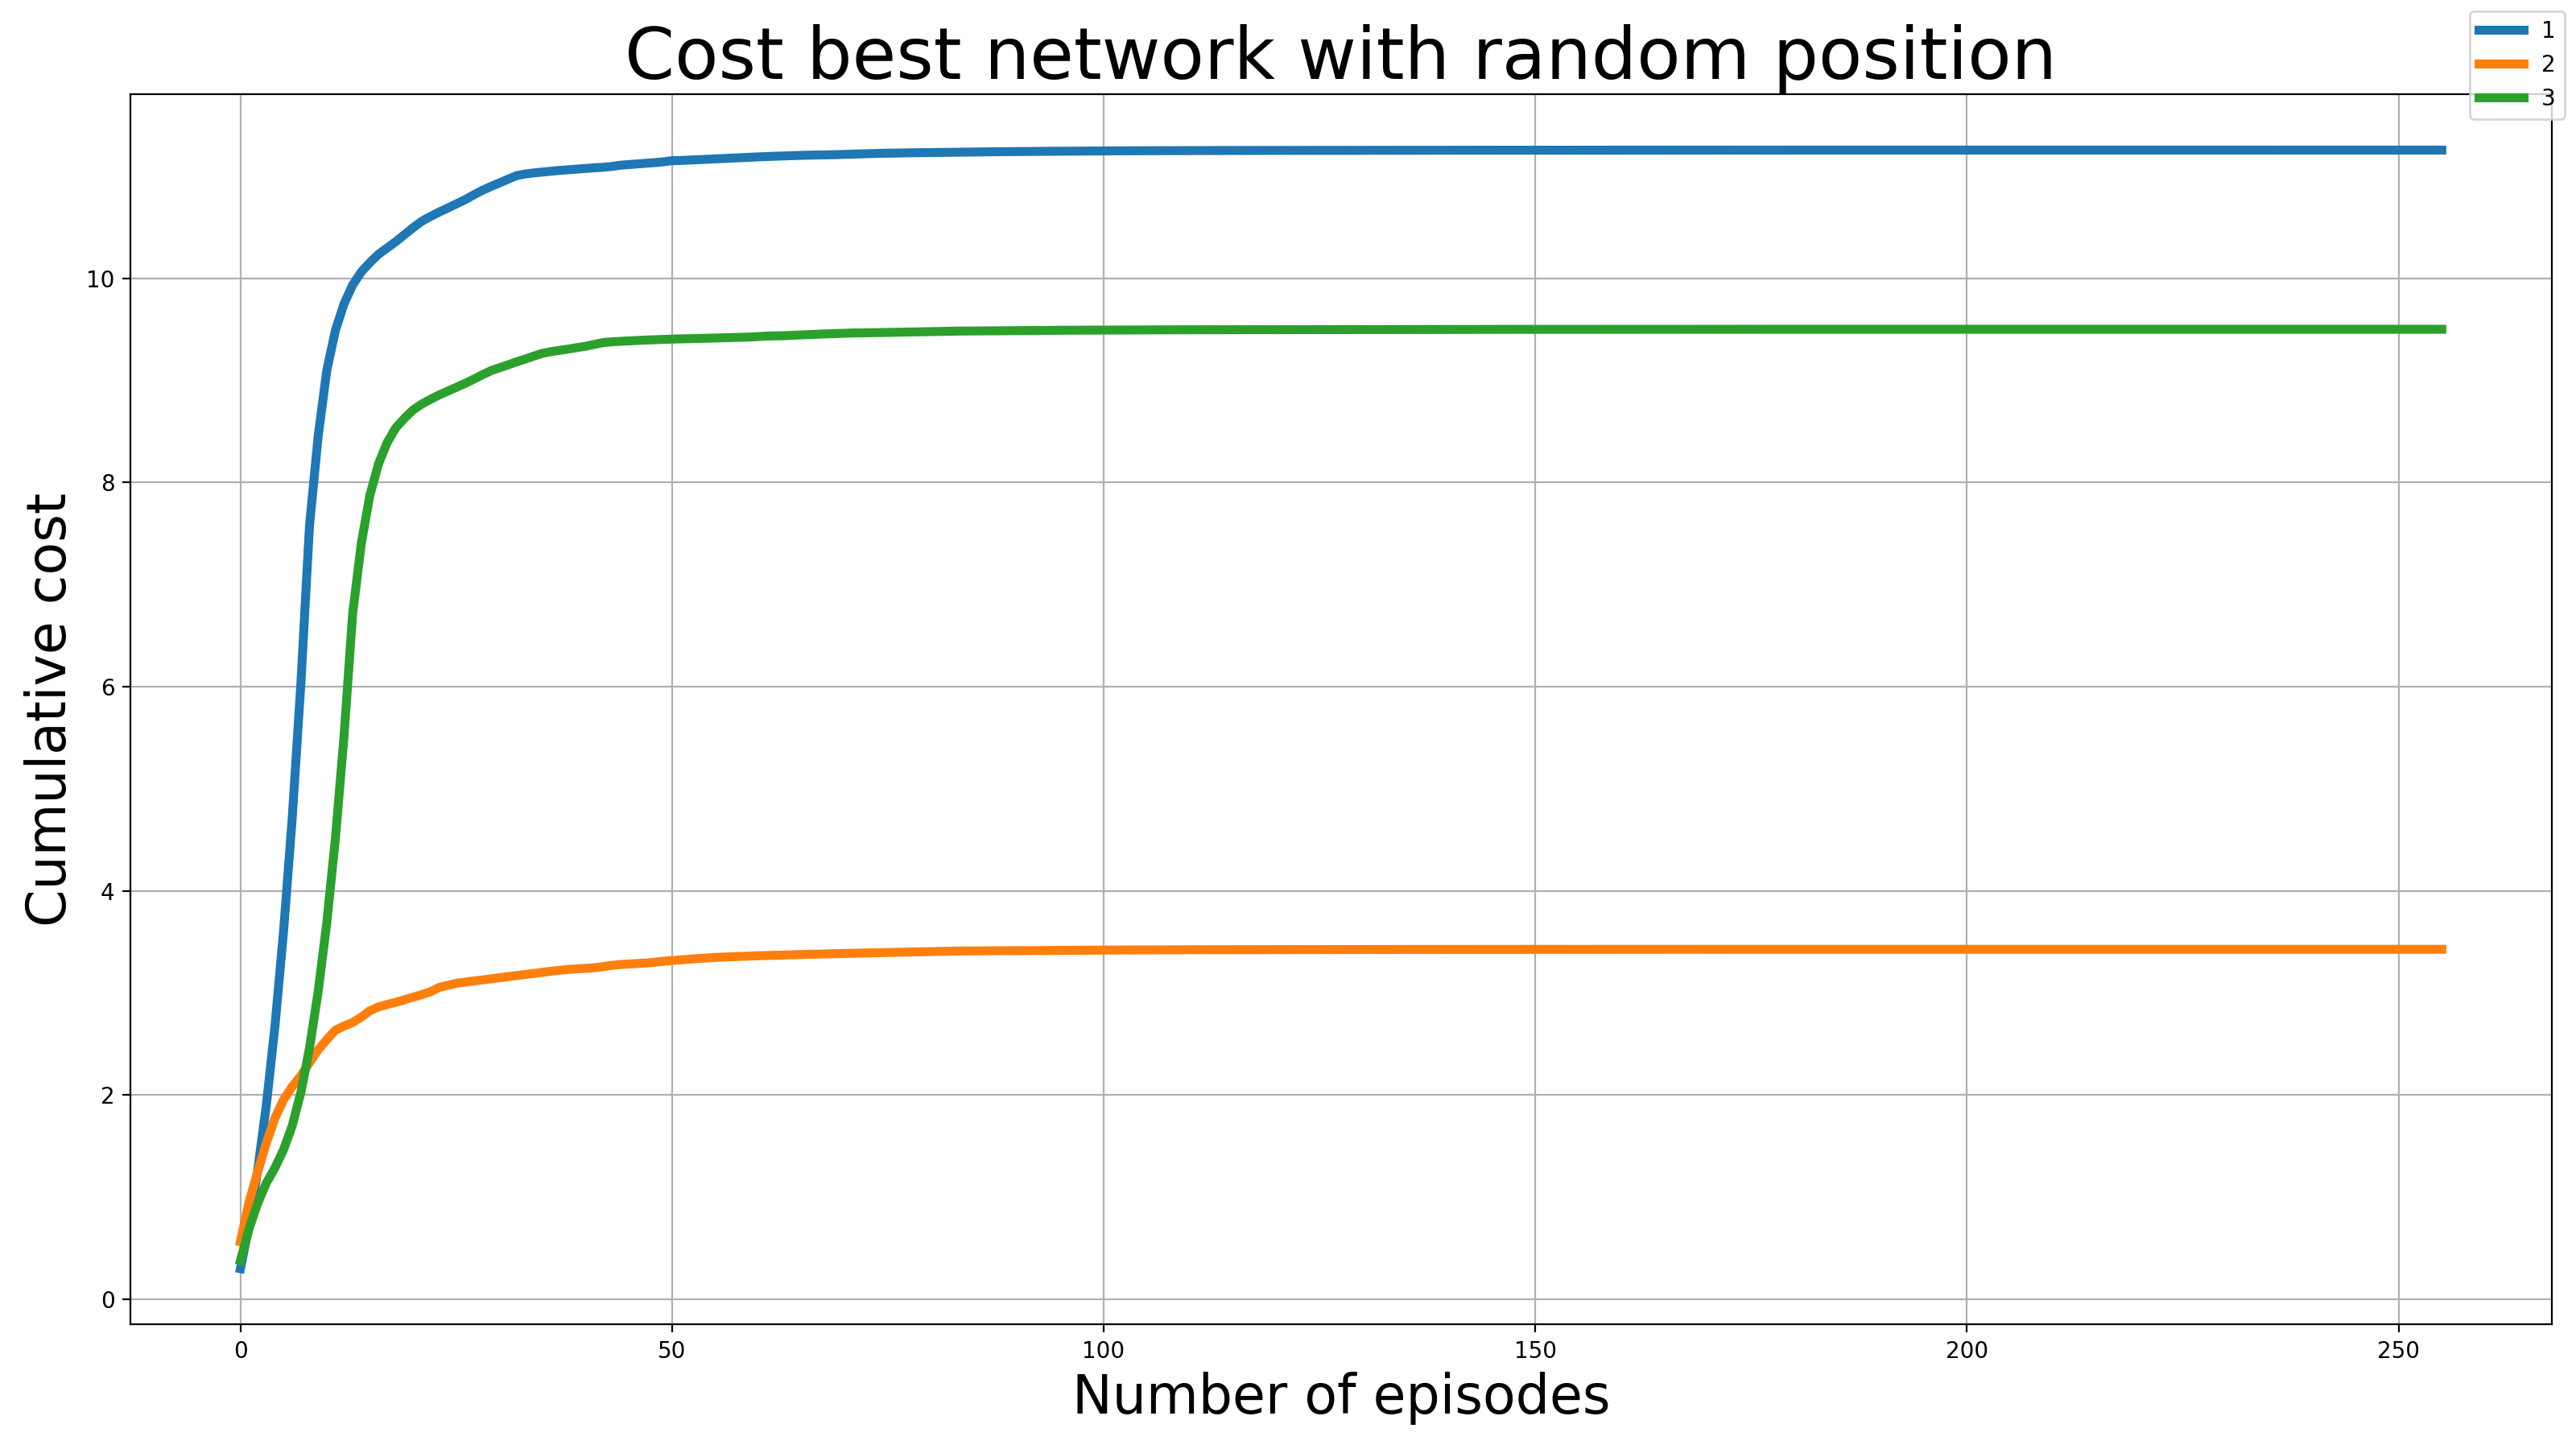
\includegraphics[width=8.5cm]{"../Figures/loss_best_net_random_positions_2J_500E_256EL.png"}
	\caption{Total cost over the test episodes for the robot starting from
			 random positions using the best performing network.}
\end{figure}
\vspace{-0.5cm}
\label{fig:Test_2_best_down_pos}
\begin{figure}[H]
	\centering
	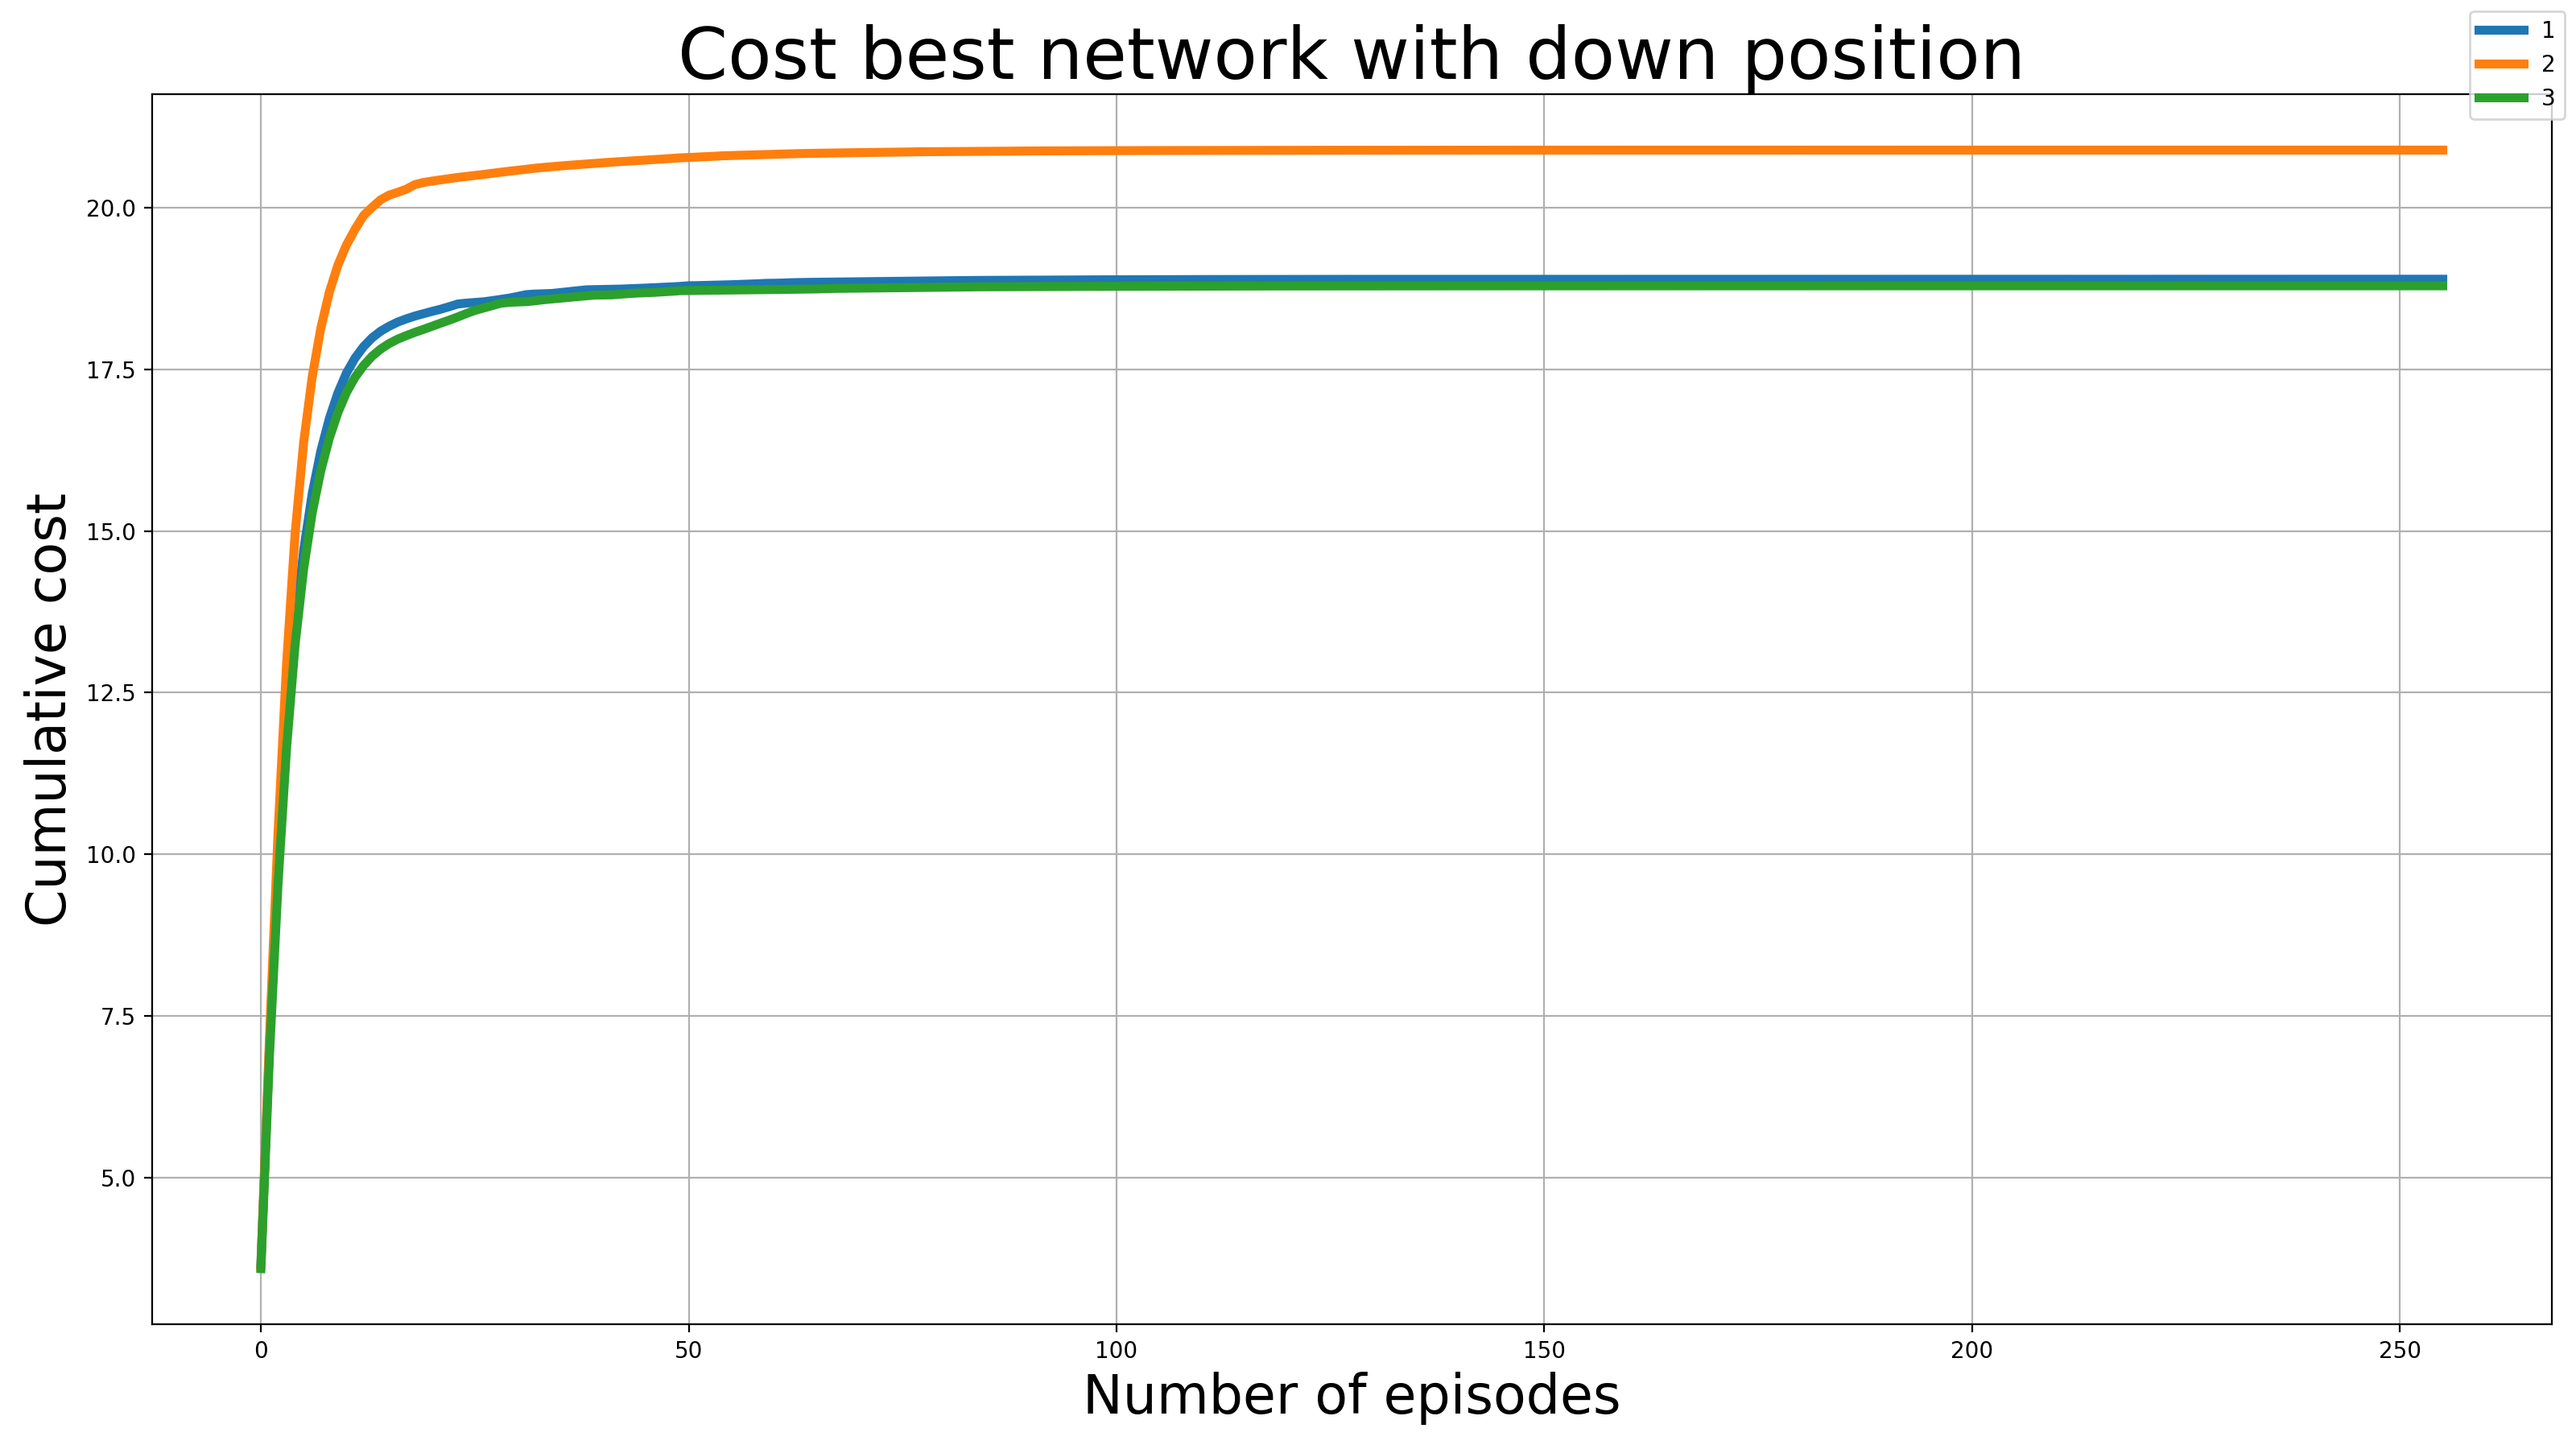
\includegraphics[width=8.5cm]{"../Figures/loss_best_net_down_positions_2J_500E_256EL.png"}
	\caption{Total cost over the test episodes for the robot starting from
			 down positions using the best performing network.}
\end{figure}


\subsection{N joints}

\subsection{General remarks}
As shown in figures \ref{fig:TrainLoss1}, \ref{fig:TrainLoss2}
we can observe how the loss during
training shows a progressive reduction with the increasing number of episodes.
The spikes in the graph has to be attributed to the exploration task that
is conducted by the policy.

In the testing phase it is possible to observe that the cumulative cost
saturates meaning that the robot is performing actions leading to the best
solution possible which is returning a cost almost 0.

Regarding the training time plots, it is possible to observe how independently
by the number of joints the time required for the computations saturates
without exceeding the 0.8 seconds per episode.
\newpage
\section{Conclusions}

\begin{thebibliography}{9}
	\bibitem{Mnih}
	Mnih, V., Kavukcuoglu, K., Silver, D. et al. Human-level control through
	deep reinforcement learning. Nature 518, 529–533 (2015).
	https://doi.org/10.1038/nature14236
\end{thebibliography}

\end{document}
